\chapter{II. Fázis: Teljes tanítás}
    Ebben a fázisban minden modellt teljesen betanítottam a teljes 144600 képet tartalmazó tanítóhalmazon. A tanítás során 10 epochon keresztül zajlott a modell optimalizálása, kivéve a NASNet modellt, ahol a számítási kapacitás korlátai miatt csak 2 epochig tartott a tréning.
    
    \textbf{Cél:} A modellek maximális, hosszú távú tanulási potenciáljának feltérképezése az egész adathalmazon.

    \section{ResNet50}
        \subsubsection{ResNet50 teljes tanítás folyamata}
        \begin{figure}[H]
        \centering
        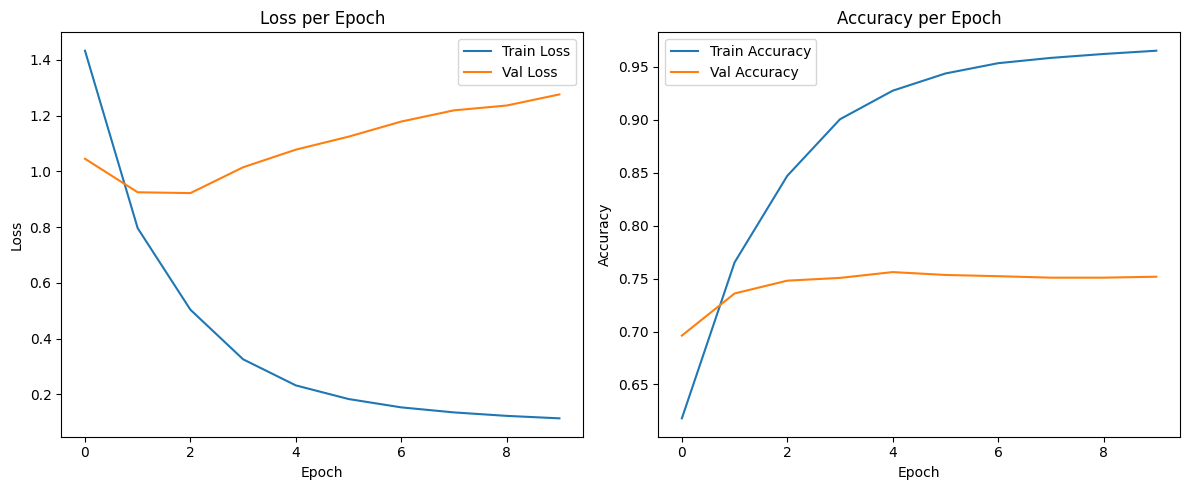
\includegraphics[width=1.0\textwidth]{images/phase02/ResNet50_learning_curve.png}
        \caption{ResNet50 teljes tanítás utáni sima Confusion Mátrix}
        \label{fig:phase02_ResNet50_learning_curves}
        \end{figure}
  
        \subsubsection{ResNet50 teljes tanítás utáni eredményei}
        \begin{center}
        \begin{longtable}{l c}
        \caption{ResNet50 teljes tanítás utáni vizsgálati eredményei} \label{tab:phase02_ResNet50} \\
        \toprule
        \textbf{Metrika} & \textbf{Érték} \\
        \midrule
        \endfirsthead
        \toprule
        \textbf{Metrika} & \textbf{Érték} \\
        \midrule
        \endhead
        Top-1 Accuracy & 0.7553 \\
        Top-5 Accuracy & 0.9351 \\
        Precision & 0.7110 \\
        Recall & 0.6808 \\
        F1-score & 0.6908 \\
        Inference time & 25.11 sec \\
        \bottomrule
        \end{longtable}
        \end{center}
    
        \subsubsection{ResNet50 eredményeinek összehasonlítása}
        \begin{center}
        \begin{longtable}{l c c}
        \caption{ResNet50 eredményeinek összehasonlítása} \label{tab:phase02_ResNet50_compare} \\
        \toprule
        \textbf{Metrika} & \textbf{Pretrained} & \textbf{Fine-tuned} \\
        \midrule
        \endfirsthead
        \toprule
        \textbf{Metrika} & \textbf{Pretrained} & \textbf{Fine-tuned} \\
        \midrule
        \endhead
        Top-1 Accuracy  & 0.4698 & 0.7553 \\
        Top-5 Accuracy & 0.7962 & 0.9351 \\
        Precision & 0.3934 & 0.7110 \\
        Recall & 0.3797 & 0.6808 \\
        F1-score & 0.3592 & 0.6908 \\
        Inference time & 25.21 sec & 25.11 sec \\
        \bottomrule
        \end{longtable}
        \end{center}
    
        \subsubsection{ResNet50 eredményeinek összehasonlítása}
        \begin{figure}[H]
        \centering
        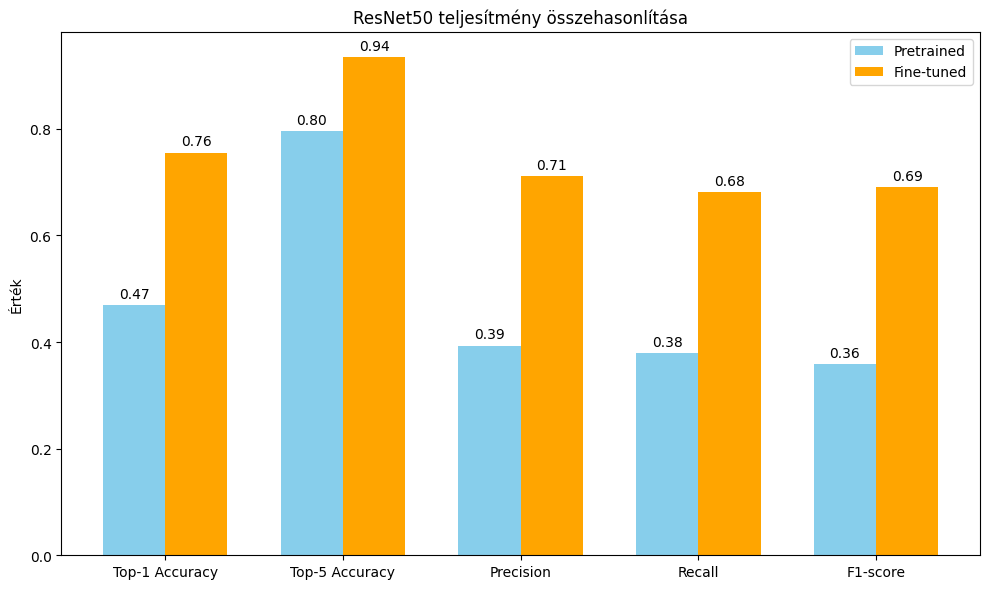
\includegraphics[width=1.0\textwidth]{images/phase02/ResNet50_compare01.png}
        \caption{ResNet50 eredményeinek összehasonlítása}
        \label{fig:ResNet50_compare01}
        \end{figure}
    
        \subsubsection{ResNet50 eredményeinek összehasonlítása}
        \begin{figure}[H]
        \centering
        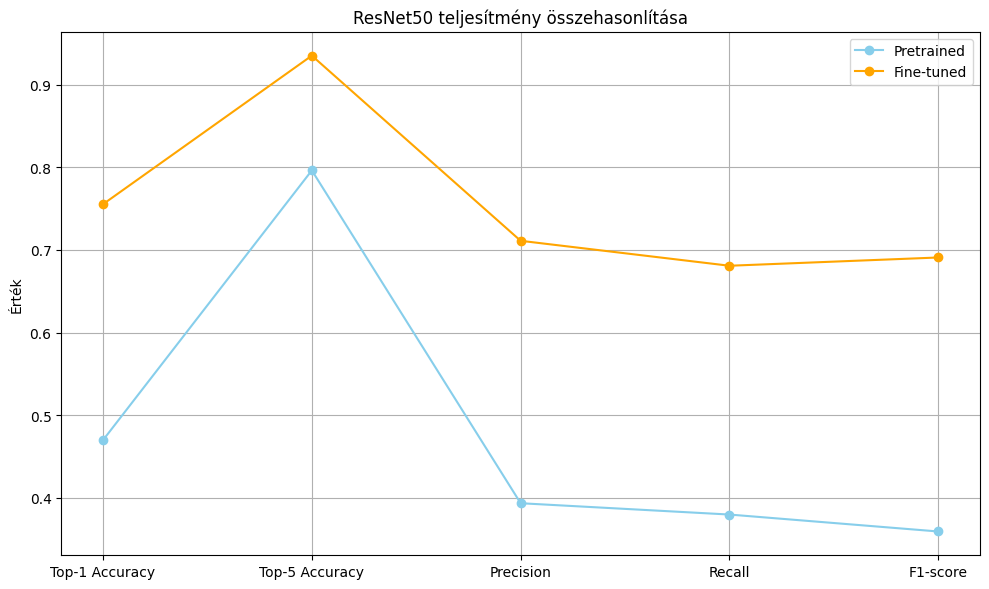
\includegraphics[width=1.0\textwidth]{images/phase02/ResNet50_compare02.png}
        \caption{ResNet50 eredményeinek összehasonlítása}
        \label{fig:ResNet50_compare02}
        \end{figure}

        \subsubsection{ResNet50 teljes tanítás utáni normalizált Confusion Mátrix}
        \begin{figure}[H]
          \centering
          
\includegraphics[width=0.8\textwidth]{images/phase02/ResNet50_normalised_conf_mat.png}
          \caption{ResNet50 teljes tanítás utáni normalizált Confusion Mátrix}
          \label{fig:phase02_ResNet50_normalised_conf_mat}
        \end{figure}
      
        \subsubsection{ResNet50 normalizált Confusion Mátrixok összehasonlítása}
        \begin{figure}[H]
          \centering
          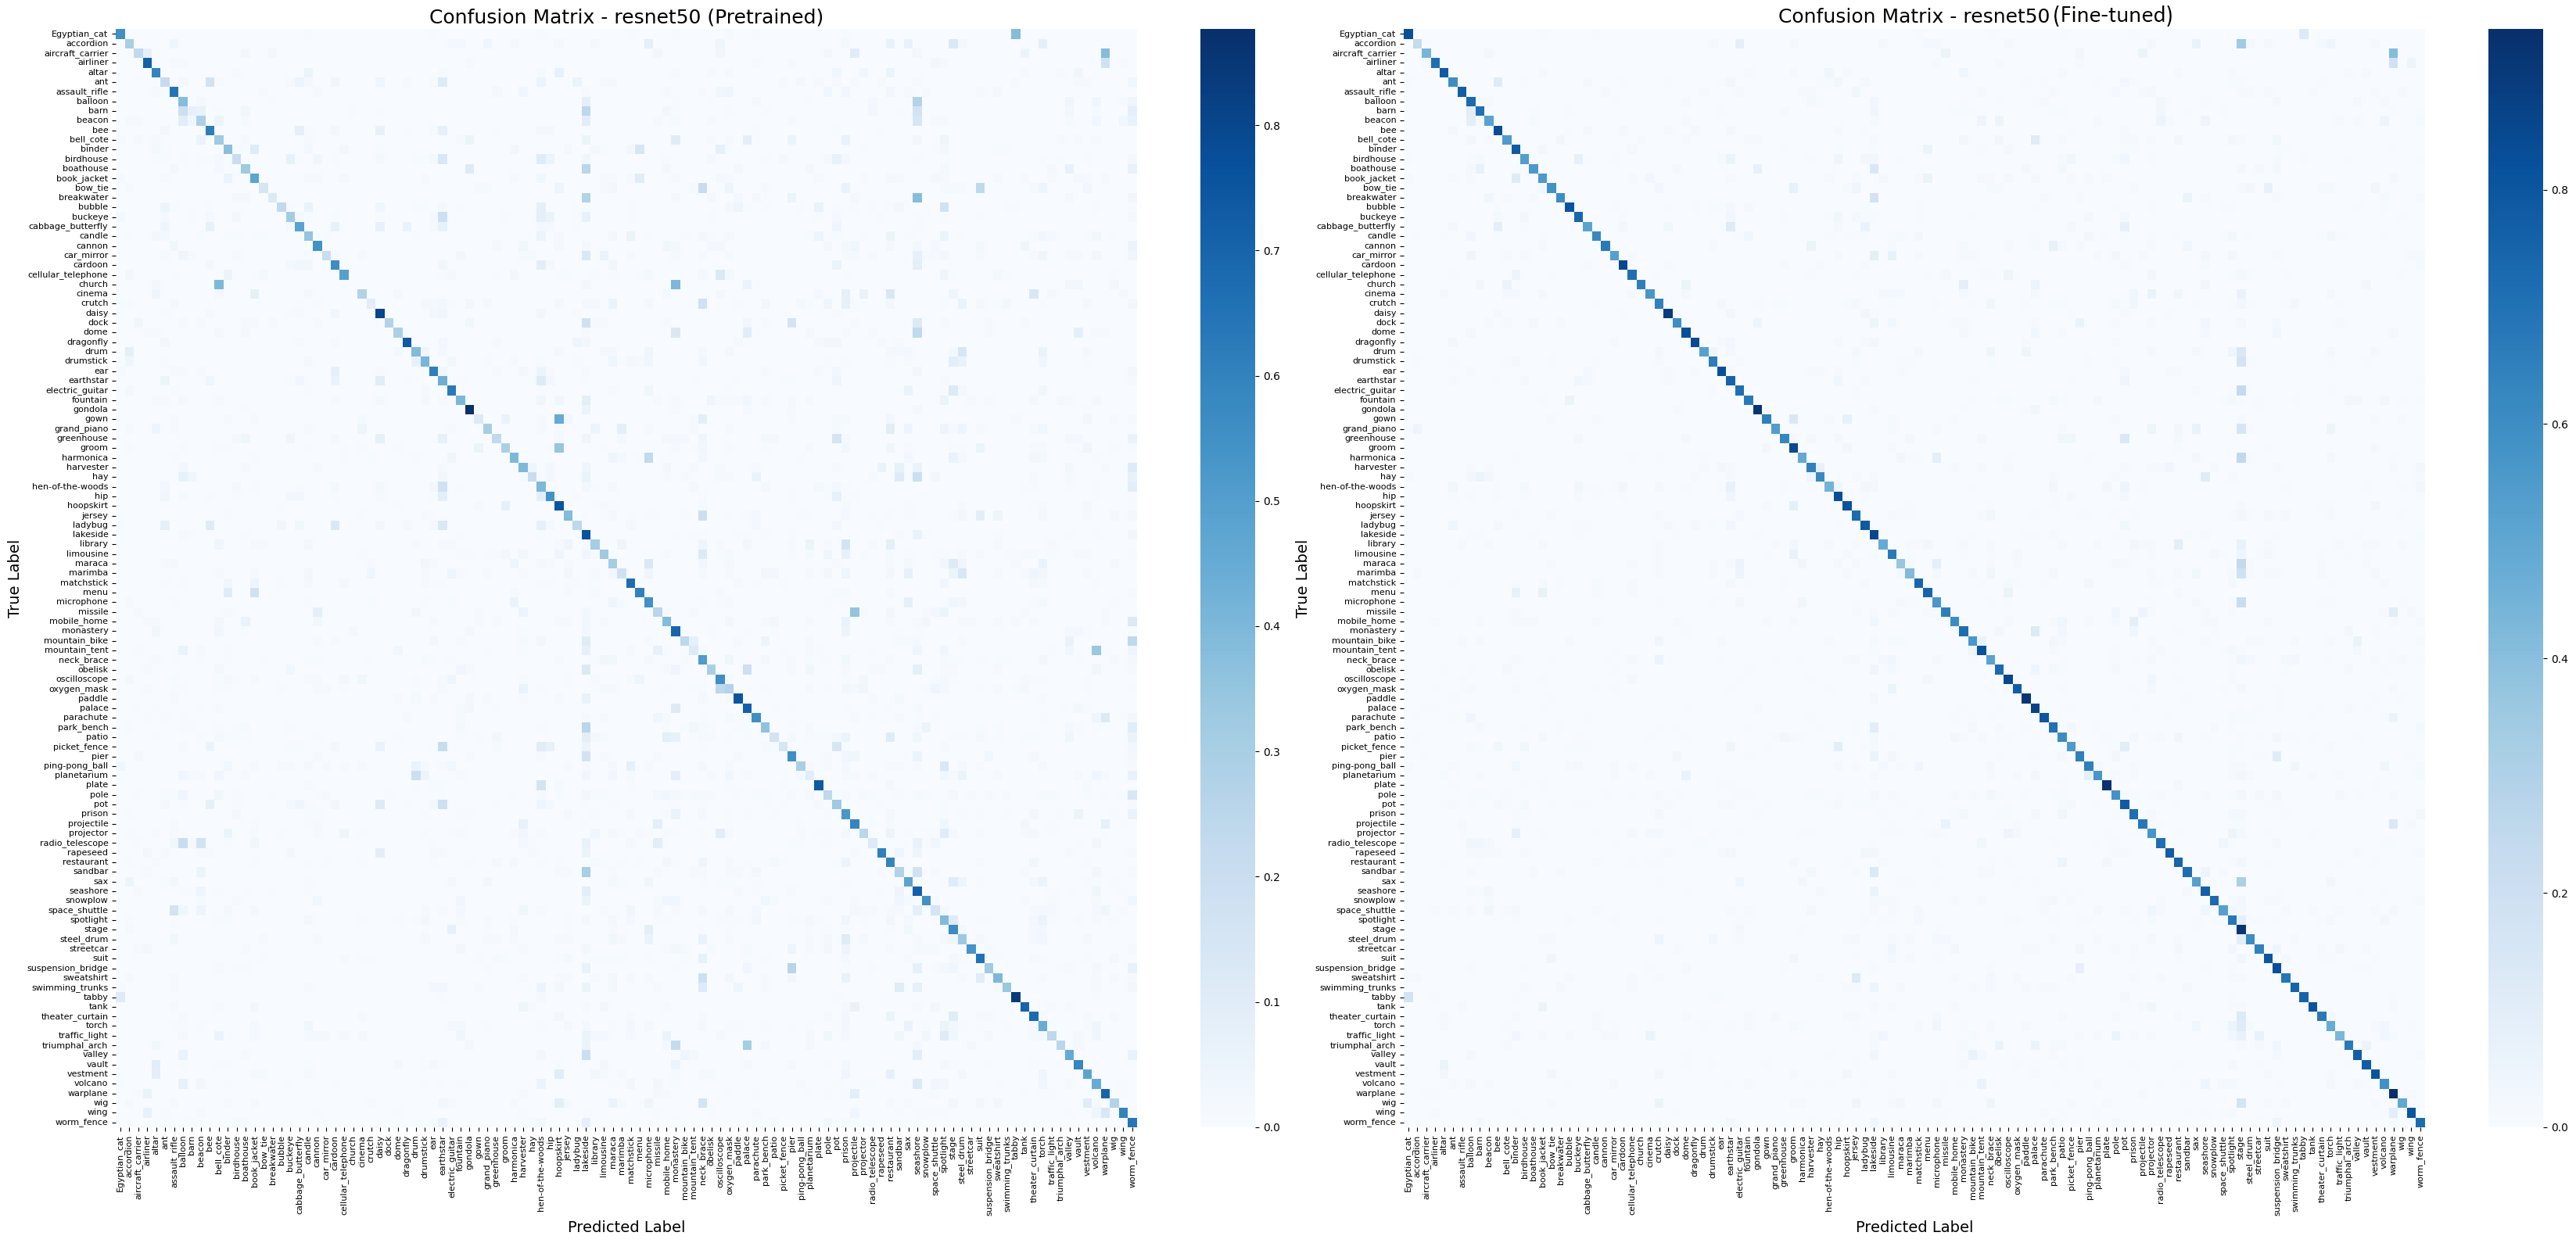
\includegraphics[width=1.0\textwidth]{images/phase02/ResNet50_normalised_conf_mat_compare.png}
          \caption{ResNet50 normalizált Confusion Mátrixok összehasonlítása}
          \label{fig:phase02_ResNet50_normalised_conf_mat_compare}
        \end{figure}

    \section{DenseNet121}
    \subsubsection{DenseNet121 teljes tanítás folyamata}
    \begin{figure}[H]
      \centering
      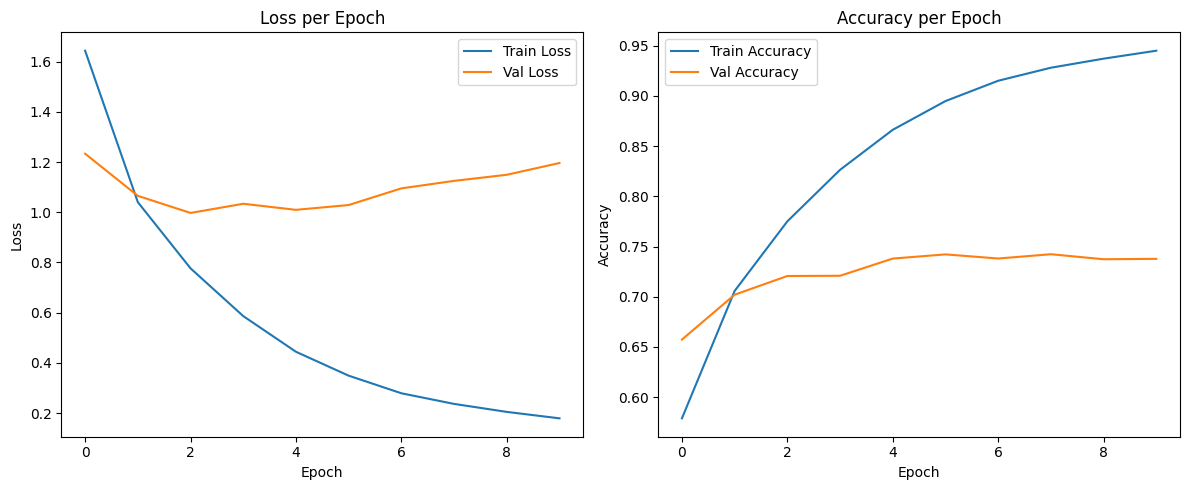
\includegraphics[width=1.0\textwidth]{images/phase02/DenseNet121_learning_curve.png}
      \caption{DenseNet121 teljes tanítás utáni sima Confusion Mátrix}
      \label{fig:phase02_DenseNet121_learning_curves}
    \end{figure}
  
  \subsubsection{DenseNet121 teljes tanítás utáni eredményei}
    \begin{center}
    \begin{longtable}{l c}
    \caption{DenseNet121 teljes tanítás utáni vizsgálati eredményei} \label{tab:phase02_DenseNet121} \\
    \toprule
    \textbf{Metrika} & \textbf{Érték} \\
    \midrule
    \endfirsthead
    \toprule
    \textbf{Metrika} & \textbf{Érték} \\
    \midrule
    \endhead
    Top-1 Accuracy & 0.7400 \\
    Top-5 Accuracy & 0.9266 \\
    Precision & 0.6811 \\
    Recall & 0.6808 \\
    F1-score & 0.6696 \\
    Inference time & 25.23 sec \\
    \bottomrule
    \end{longtable}
    \end{center}
  
  \subsubsection{DenseNet121 eredményeinek összehasonlítása}
    \begin{center}
    \begin{longtable}{l c c}
    \caption{DenseNet121 eredményeinek összehasonlítása} \label{tab:phase02_DenseNet121_compare} \\
    \toprule
    \textbf{Metrika} & \textbf{Pretrained} & \textbf{Fine-tuned} \\
    \midrule
    \endfirsthead
    \toprule
    \textbf{Metrika} & \textbf{Pretrained} & \textbf{Fine-tuned} \\
    \midrule
    \endhead
    Top-1 Accuracy  & 0.4498 & 0.7400 \\
    Top-5 Accuracy & 0.7806 & 0.9266 \\
    Precision & 0.3874 & 0.6811 \\
    Recall & 0.3611 & 0.6680 \\
    F1-score & 0.3408 & 0.6696 \\
    Inference time & 25.15 sec & 25.23 sec \\
    \bottomrule
    \end{longtable}
    \end{center}
  
  \subsubsection{DenseNet121 eredményeinek összehasonlítása}
    \begin{figure}[H]
      \centering
      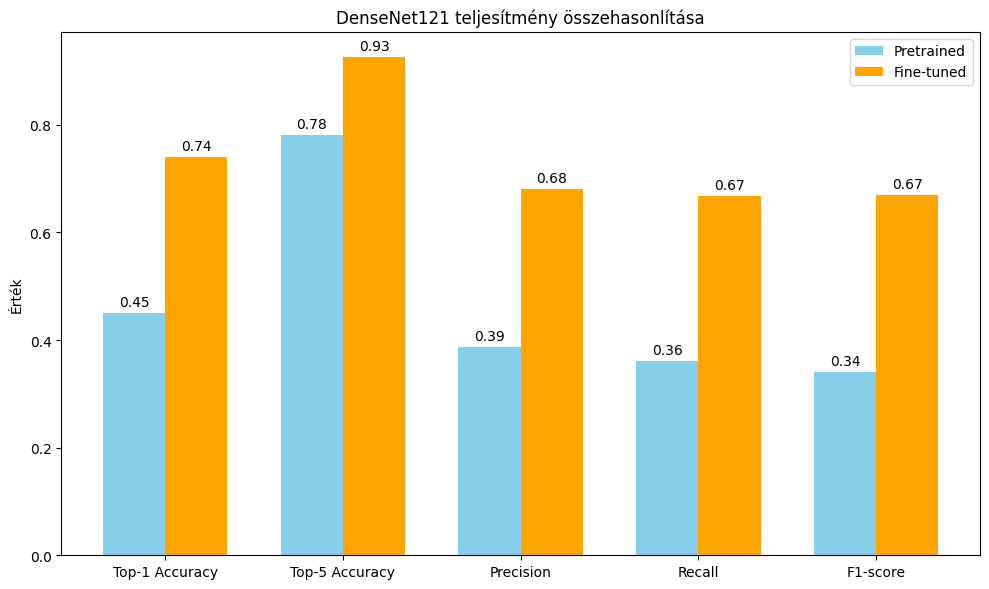
\includegraphics[width=1.0\textwidth]{images/phase02/DenseNet121_compare01.png}
      \caption{DenseNet121 eredményeinek összehasonlítása}
      \label{fig:DenseNet121_compare01}
    \end{figure}
  
  \subsubsection{DenseNet121 eredményeinek összehasonlítása}
    \begin{figure}[H]
      \centering
      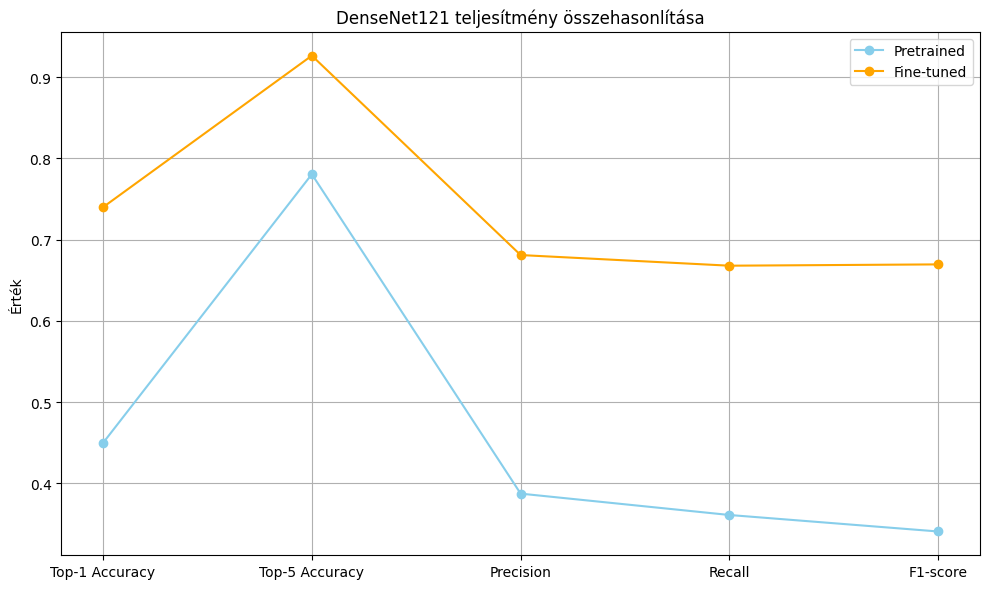
\includegraphics[width=1.0\textwidth]{images/phase02/DenseNet121_compare02.png}
      \caption{DenseNet121 eredményeinek összehasonlítása}
      \label{fig:DenseNet121_compare02}
    \end{figure}

    \subsubsection{DenseNet121 teljes tanítás utáni normalizált Confusion Mátrix}
    \begin{figure}[H]
      \centering
      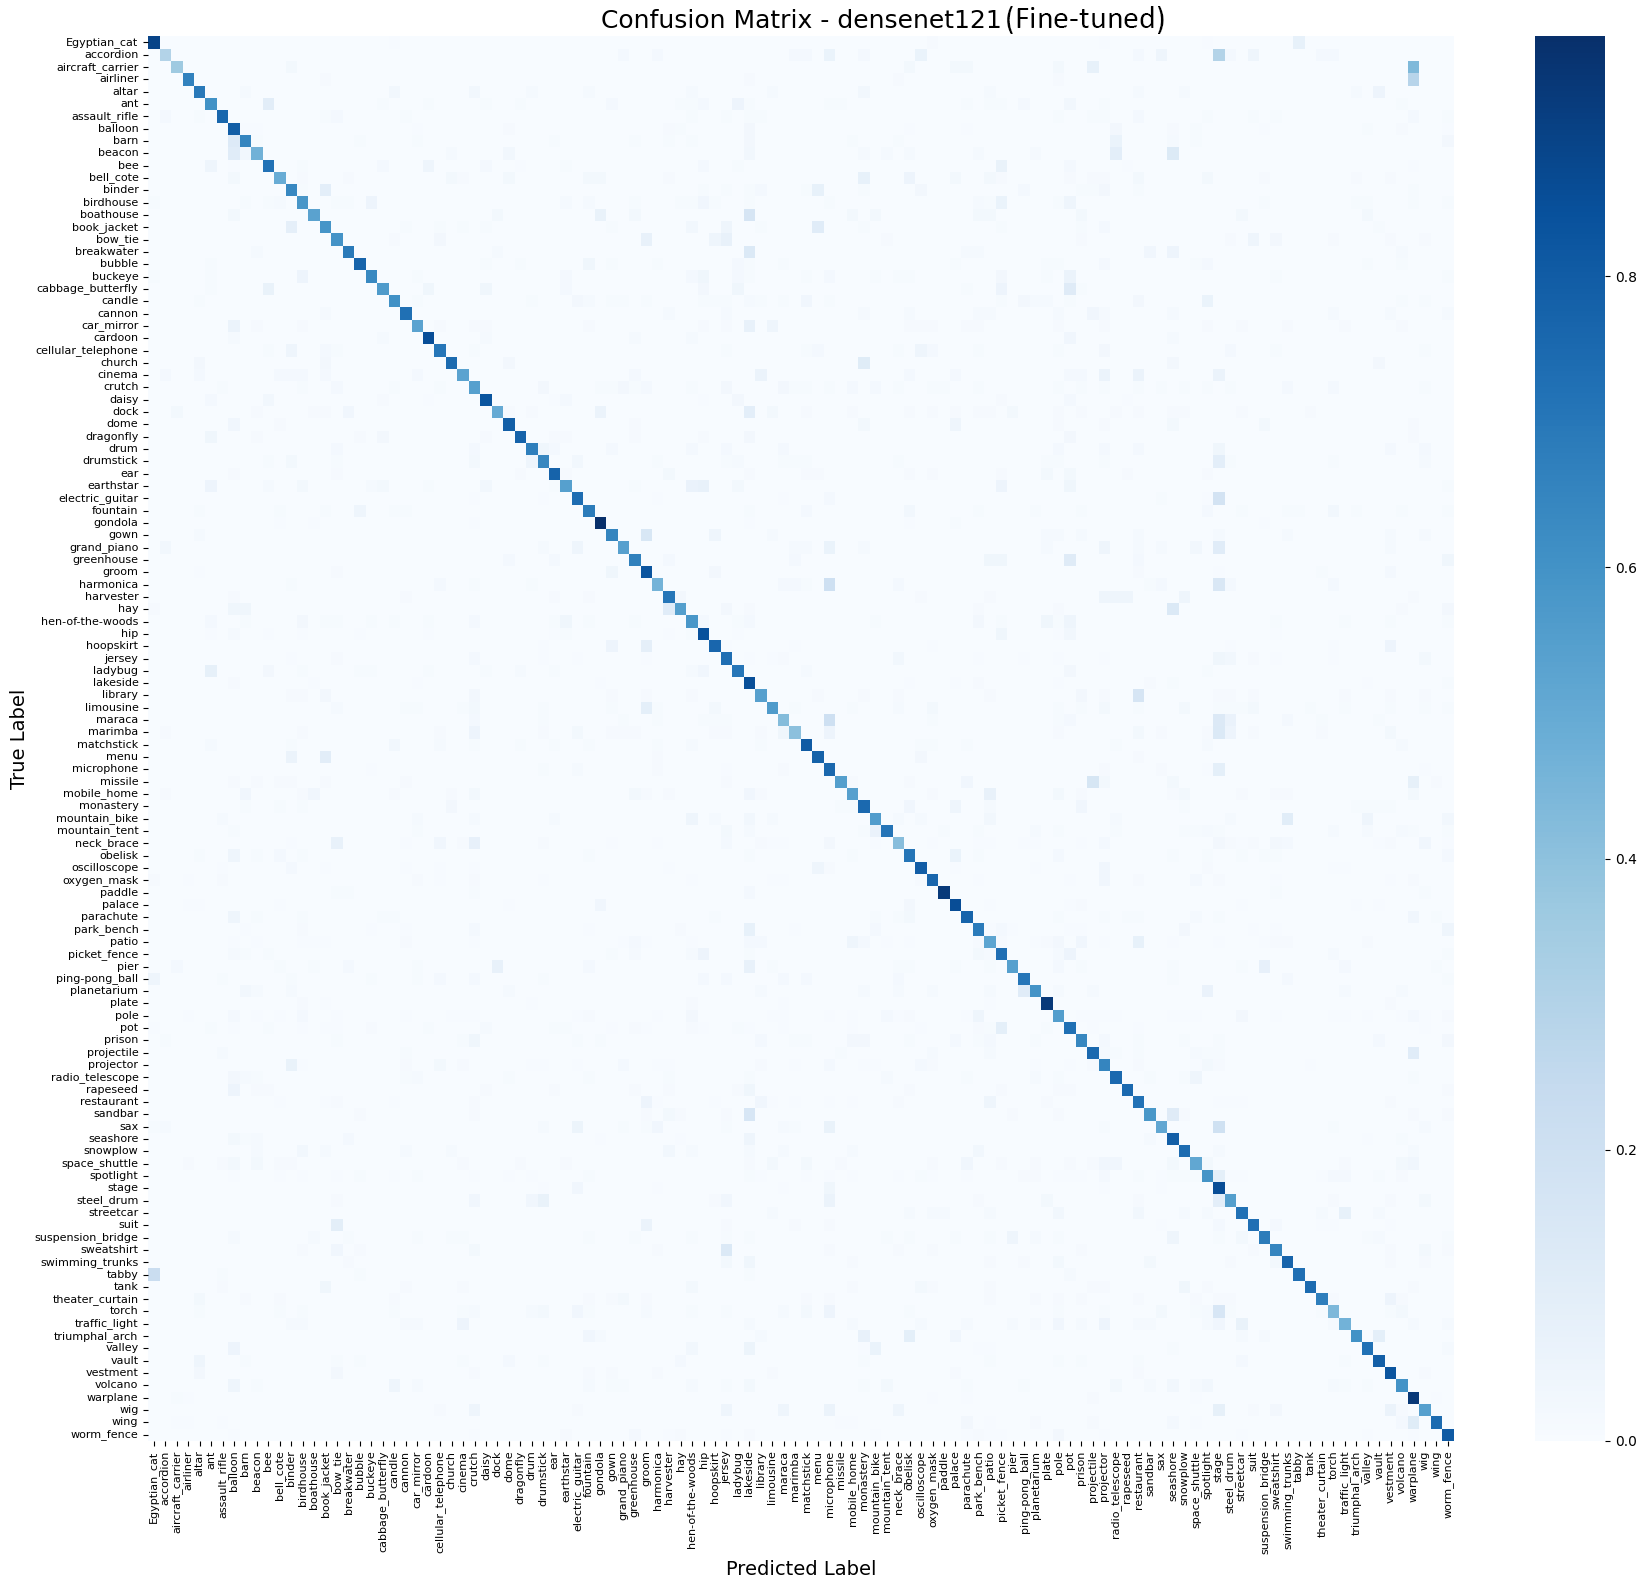
\includegraphics[width=0.8\textwidth]{images/phase02/phase02_DenseNet121_normalised_conf_mat.png}
      \caption{DenseNet121 teljes tanítás utáni normalizált Confusion Mátrix}
      \label{fig:phase02_DenseNet121_normalised_conf_mat}
    \end{figure}
  
    \subsubsection{DenseNet121 normalizált Confusion Mátrixok összehasonlítása}
    \begin{figure}[H]
      \centering
      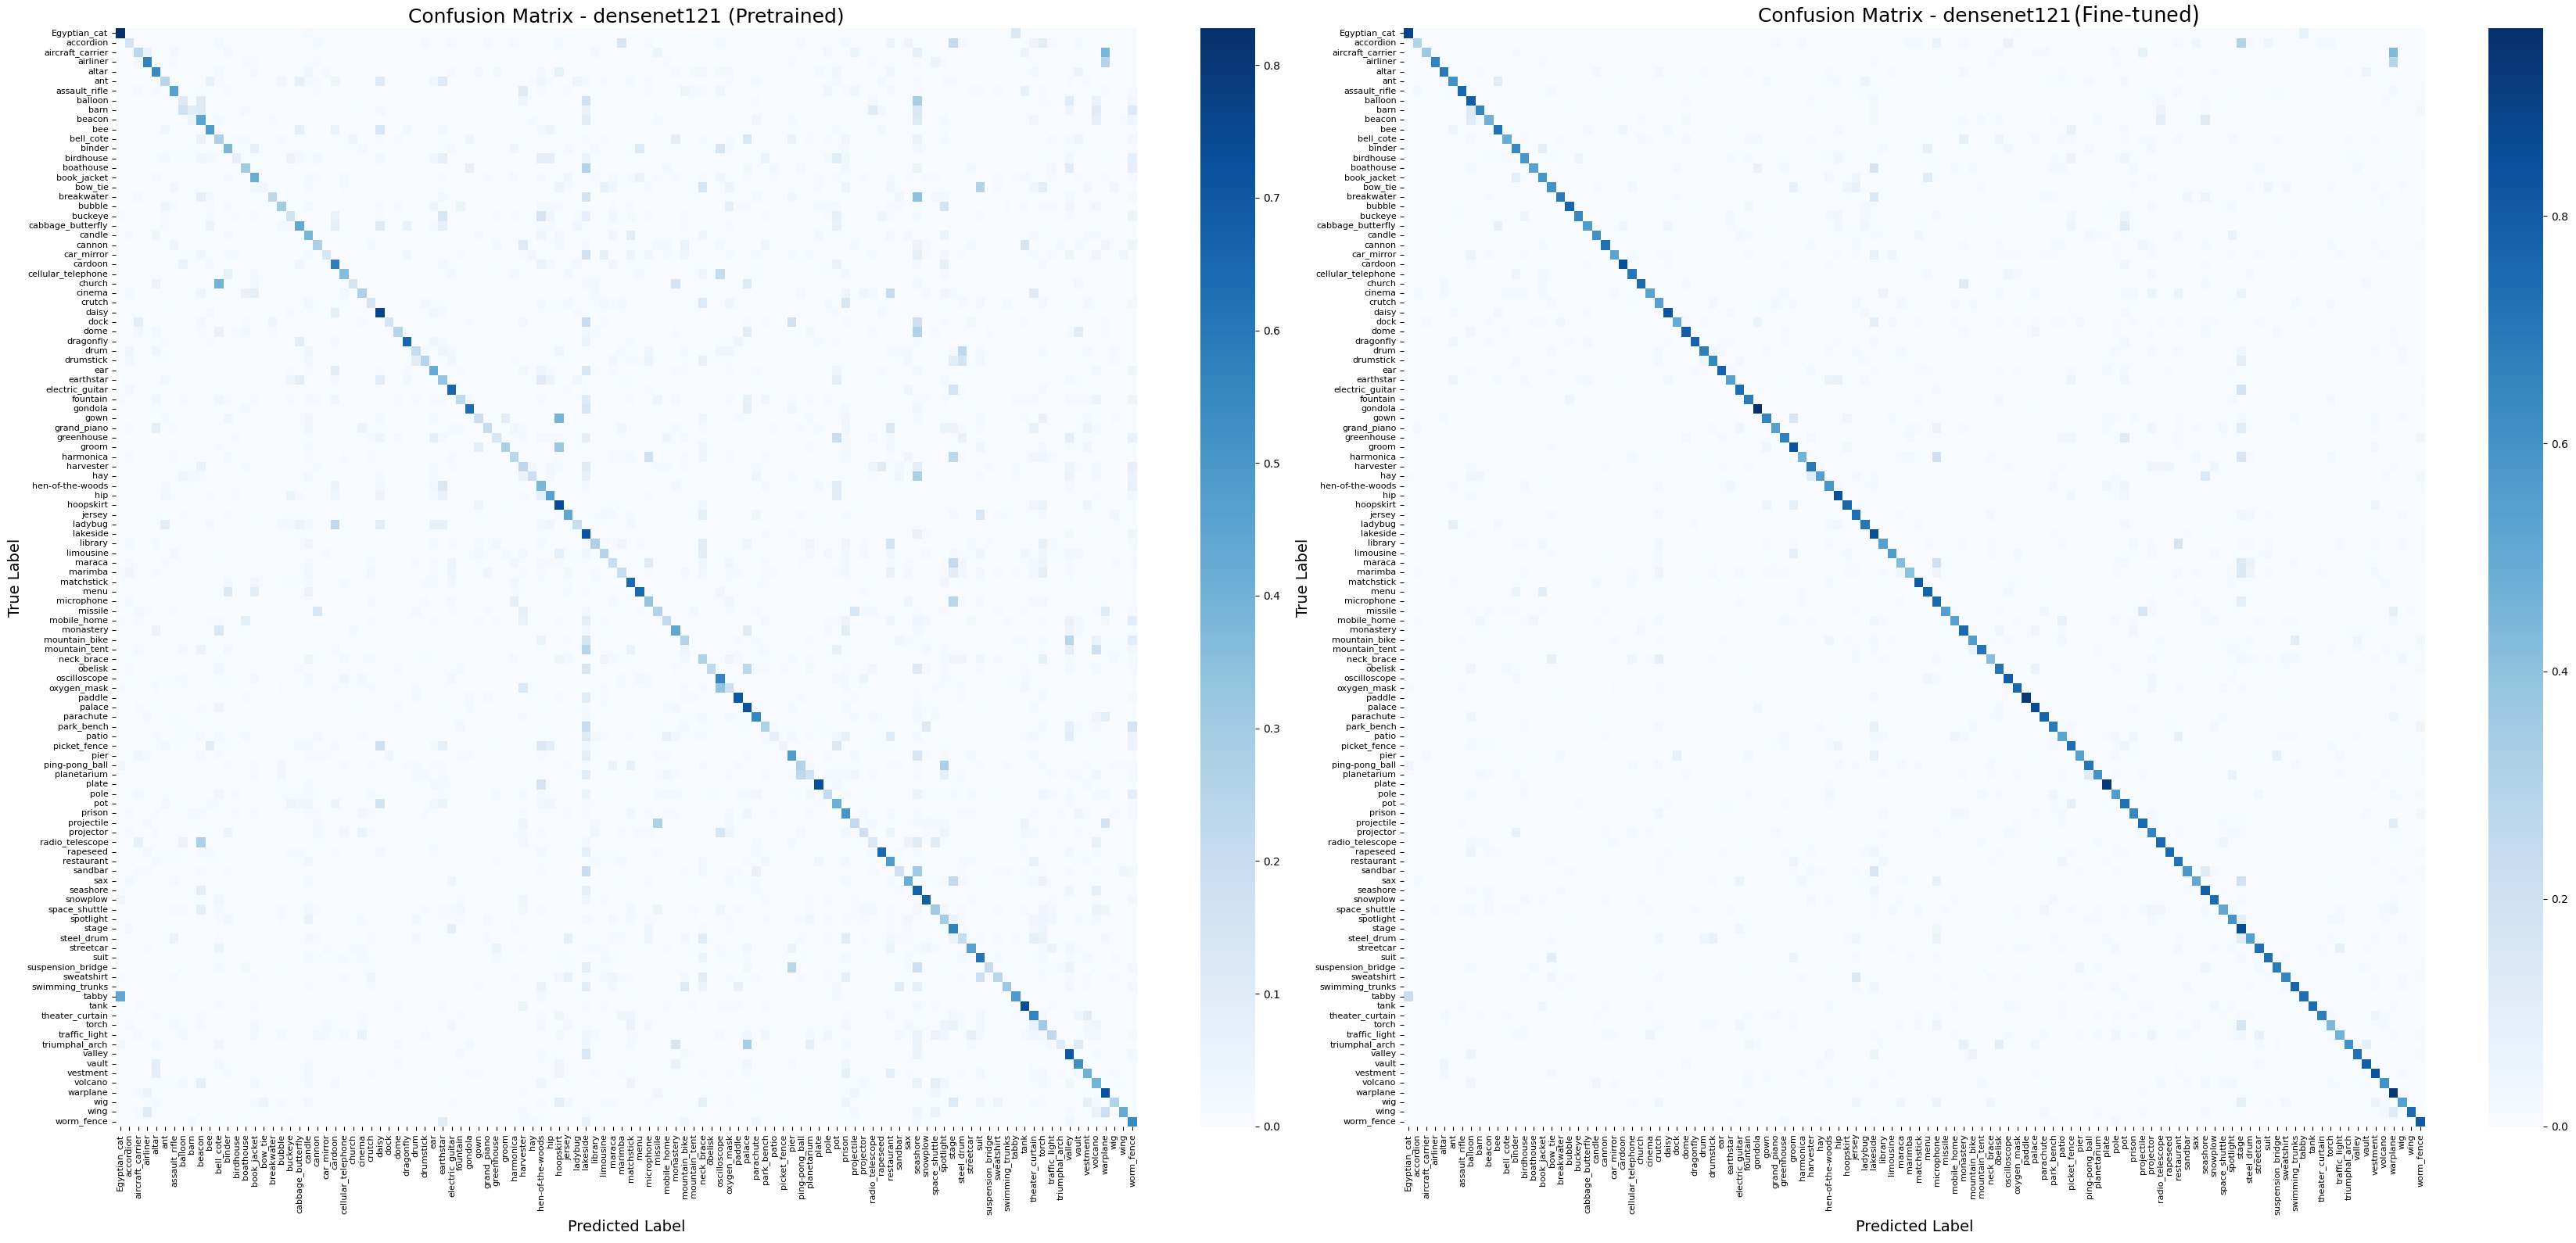
\includegraphics[width=1.0\textwidth]{images/phase02/phase02_DenseNet121_normalised_conf_mat_compare.png}
      \caption{DenseNet121 normalizált Confusion Mátrixok összehasonlítása}
      \label{fig:phase02_DenseNet121_normalised_conf_mat_compare}
    \end{figure}

    \section{EfficientNet-B0}
    \subsubsection{EfficientNet-B0 teljes tanítás folyamata}
    \begin{figure}[H]
      \centering
      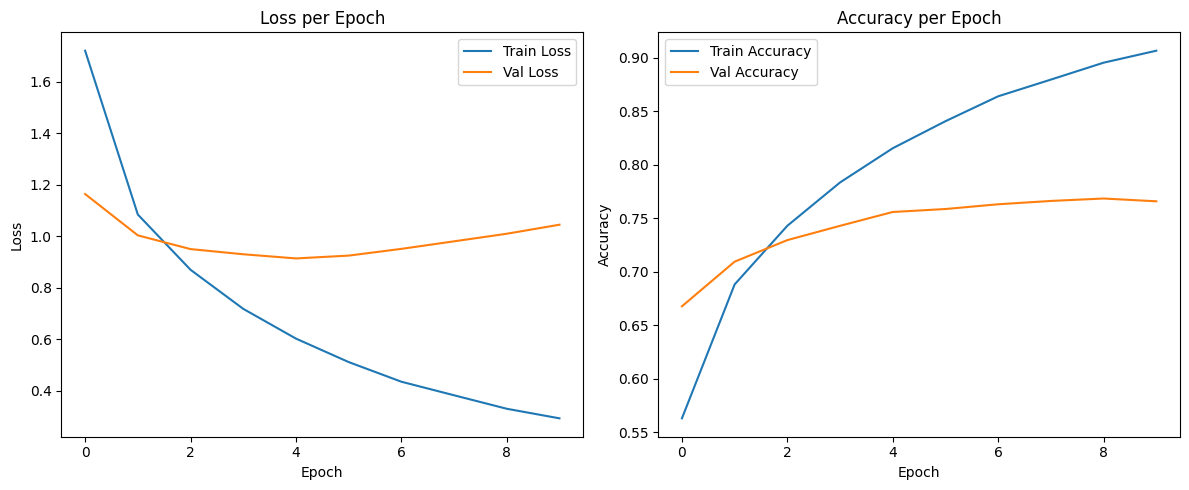
\includegraphics[width=1.0\textwidth]{images/phase02/EfficientNet-B0_learning_curve.png}
      \caption{EfficientNet-B0 teljes tanítás utáni sima Confusion Mátrix}
      \label{fig:phase02_EfficientNet-B0_learning_curves}
    \end{figure}
  
  \subsubsection{EfficientNet-B0 teljes tanítás utáni eredményei}
    \begin{center}
    \begin{longtable}{l c}
    \caption{EfficientNet-B0 teljes tanítás utáni vizsgálati eredményei} \label{tab:phase02_EfficientNet-B0} \\
    \toprule
    \textbf{Metrika} & \textbf{Érték} \\
    \midrule
    \endfirsthead
    \toprule
    \textbf{Metrika} & \textbf{Érték} \\
    \midrule
    \endhead
    Top-1 Accuracy & 0.7649 \\
    Top-5 Accuracy & 0.9421 \\
    Precision & 0.7130 \\
    Recall & 0.6950 \\
    F1-score & 0.7001 \\
    Inference time & 25.26 sec \\
    \bottomrule
    \end{longtable}
    \end{center}
  
  \subsubsection{EfficientNet-B0 eredményeinek összehasonlítása}
    \begin{center}
    \begin{longtable}{l c c}
    \caption{EfficientNet-B0 eredményeinek összehasonlítása} \label{tab:phase02_EfficientNet-B0_compare} \\
    \toprule
    \textbf{Metrika} & \textbf{Pretrained} & \textbf{Fine-tuned} \\
    \midrule
    \endfirsthead
    \toprule
    \textbf{Metrika} & \textbf{Pretrained} & \textbf{Fine-tuned} \\
    \midrule
    \endhead
    Top-1 Accuracy  & 0.4802 & 0.7649 \\
    Top-5 Accuracy & 0.8217 & 0.9421 \\
    Precision & 0.4137 & 0.7130 \\
    Recall & 0.4039 & 0.6950 \\
    F1-score & 0.3829 & 0.7001 \\
    Inference time & 28.89 sec & 25.26 sec \\
    \bottomrule
    \end{longtable}
    \end{center}
  
  \subsubsection{EfficientNet-B0 eredményeinek összehasonlítása}
    \begin{figure}[H]
      \centering
      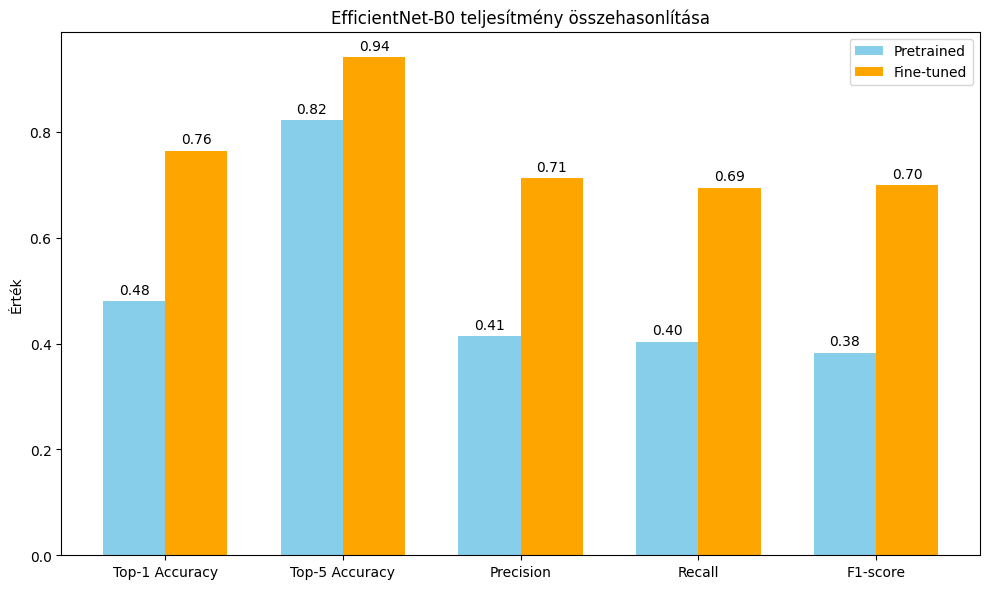
\includegraphics[width=1.0\textwidth]{images/phase02/EfficientNet-B0_compare01.png}
      \caption{EfficientNet-B0 eredményeinek összehasonlítása}
      \label{fig:EfficientNet-B0_compare01}
    \end{figure}
  
  \subsubsection{EfficientNet-B0 eredményeinek összehasonlítása}
    \begin{figure}[H]
      \centering
      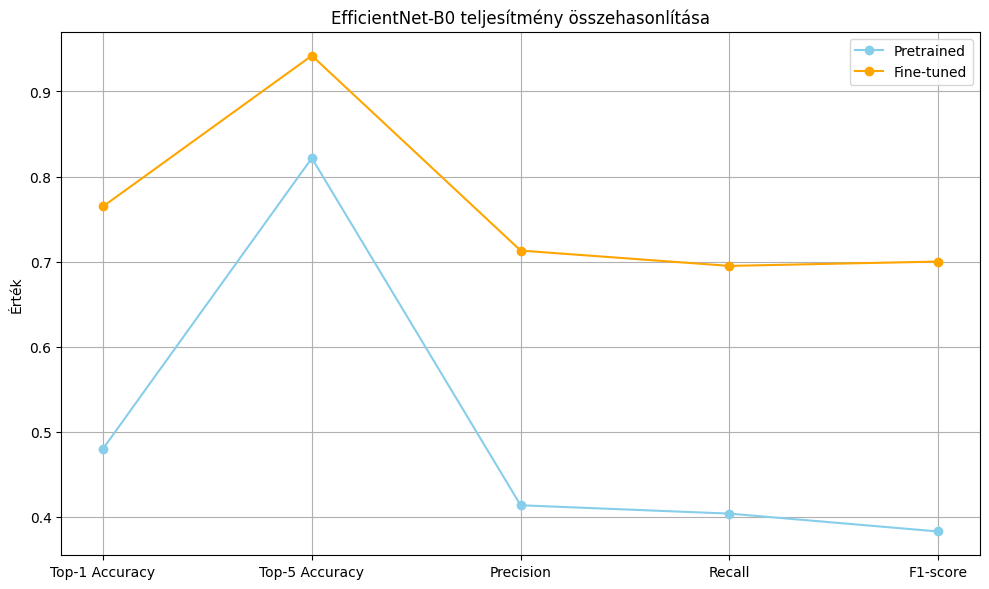
\includegraphics[width=1.0\textwidth]{images/phase02/EfficientNet-B0_compare02.png}
      \caption{EfficientNet-B0 eredményeinek összehasonlítása}
      \label{fig:EfficientNet-B0_compare02}
    \end{figure}

    \subsubsection{EfficientNet-B0 teljes tanítás utáni normalizált Confusion Mátrix}
    \begin{figure}[H]
      \centering
      
\includegraphics[width=0.8\textwidth]{images/phase02/EfficientNet-B0_normalised_conf_mat.png}
      \caption{EfficientNet-B0 teljes tanítás utáni normalizált Confusion Mátrix}
      \label{fig:phase02_EfficientNet-B0_normalised_conf_mat}
    \end{figure}
  
    \subsubsection{EfficientNet-B0 normalizált Confusion Mátrixok összehasonlítása}
    \begin{figure}[H]
      \centering
      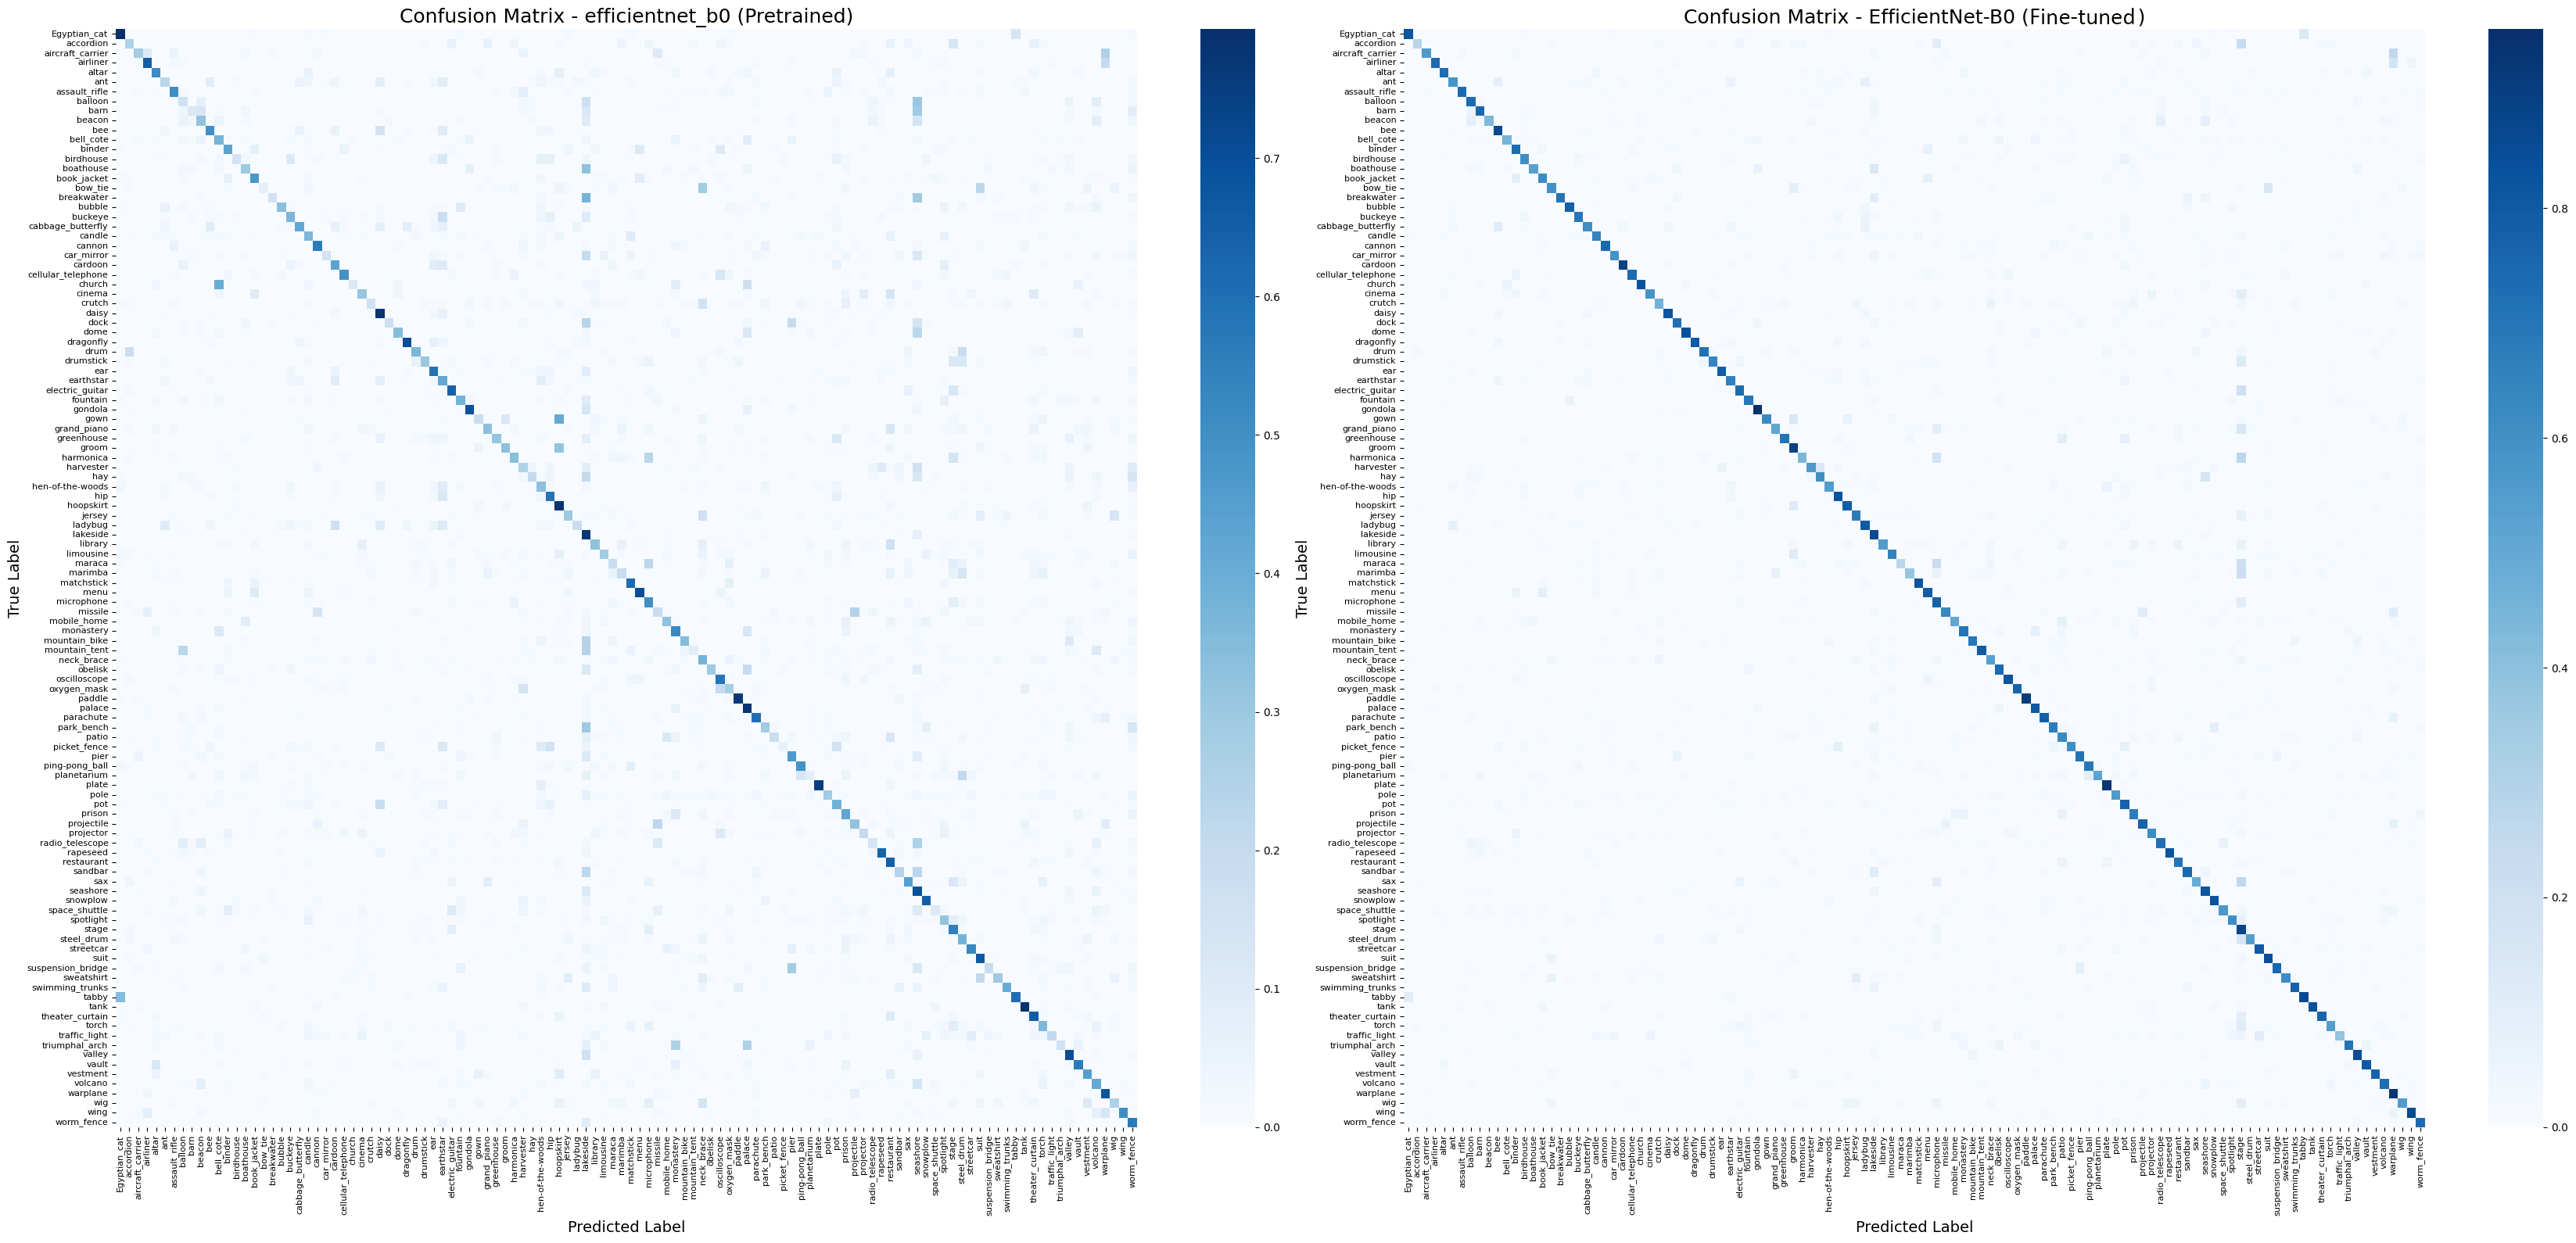
\includegraphics[width=1.0\textwidth]{images/phase02/EfficientNet-B0_normalised_conf_mat_compare.png}
      \caption{EfficientNet-B0 normalizált Confusion Mátrixok összehasonlítása}
      \label{fig:phase02_EfficientNet-B0_normalised_conf_mat_compare}
    \end{figure}

    \section{ConvNeXt-Tiny}
    \subsubsection{ConvNeXt-Tiny teljes tanítás folyamata}
    \begin{figure}[H]
      \centering
      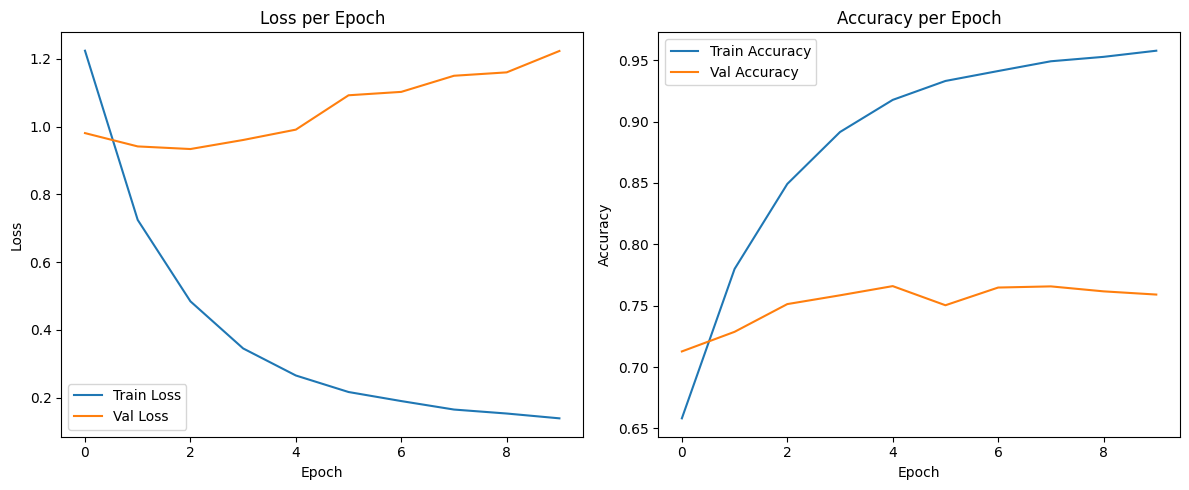
\includegraphics[width=1.0\textwidth]{images/phase02/ConvNeXt-Tiny_learning_curve.png}
      \caption{ConvNeXt-Tiny teljes tanítás utáni sima Confusion Mátrix}
      \label{fig:phase02_ConvNeXt-Tiny_learning_curves}
    \end{figure}
  
  \subsubsection{ConvNeXt-Tiny teljes tanítás utáni eredményei}
    \begin{center}
    \begin{longtable}{l c}
    \caption{ConvNeXt-Tiny teljes tanítás utáni vizsgálati eredményei} \label{tab:phase02_ConvNeXt-Tiny} \\
    \toprule
    \textbf{Metrika} & \textbf{Érték} \\
    \midrule
    \endfirsthead
    \toprule
    \textbf{Metrika} & \textbf{Érték} \\
    \midrule
    \endhead
    Top-1 Accuracy & 0.7624 \\
    Top-5 Accuracy & 0.9357 \\
    Precision & 0.7168 \\
    Recall & 0.6841 \\
    F1-score & 0.6947 \\
    Inference time & 25.67 sec \\
    \bottomrule
    \end{longtable}
    \end{center}
  
  \subsubsection{ConvNeXt-Tiny eredményeinek összehasonlítása}
    \begin{center}
    \begin{longtable}{l c c}
    \caption{ConvNeXt-Tiny eredményeinek összehasonlítása} \label{tab:phase02_ConvNeXt-Tiny_compare} \\
    \toprule
    \textbf{Metrika} & \textbf{Pretrained} & \textbf{Fine-tuned} \\
    \midrule
    \endfirsthead
    \toprule
    \textbf{Metrika} & \textbf{Pretrained} & \textbf{Fine-tuned} \\
    \midrule
    \endhead
    Top-1 Accuracy  & 0.5048 & 0.7624 \\
    Top-5 Accuracy & 0.8471 & 0.9357 \\
    Precision & 0.4917 & 0.7168 \\
    Recall & 0.4369 & 0.6841 \\
    F1-score & 0.4194 & 0.6947 \\
    Inference time & 38.40 sec & 25.67 sec \\
    \bottomrule
    \end{longtable}
    \end{center}
  
  \subsubsection{ConvNeXt-Tiny eredményeinek összehasonlítása}
    \begin{figure}[H]
      \centering
      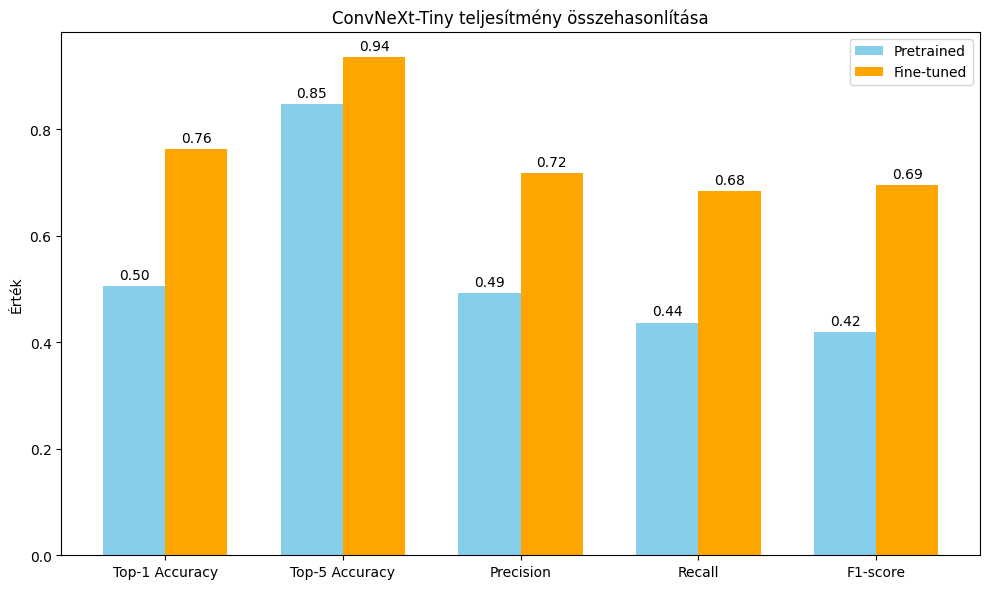
\includegraphics[width=1.0\textwidth]{images/phase02/ConvNeXt-Tiny_compare01.png}
      \caption{ConvNeXt-Tiny eredményeinek összehasonlítása}
      \label{fig:ConvNeXt-Tiny_compare01}
    \end{figure}
  
  \subsubsection{ConvNeXt-Tiny eredményeinek összehasonlítása}
    \begin{figure}[H]
      \centering
      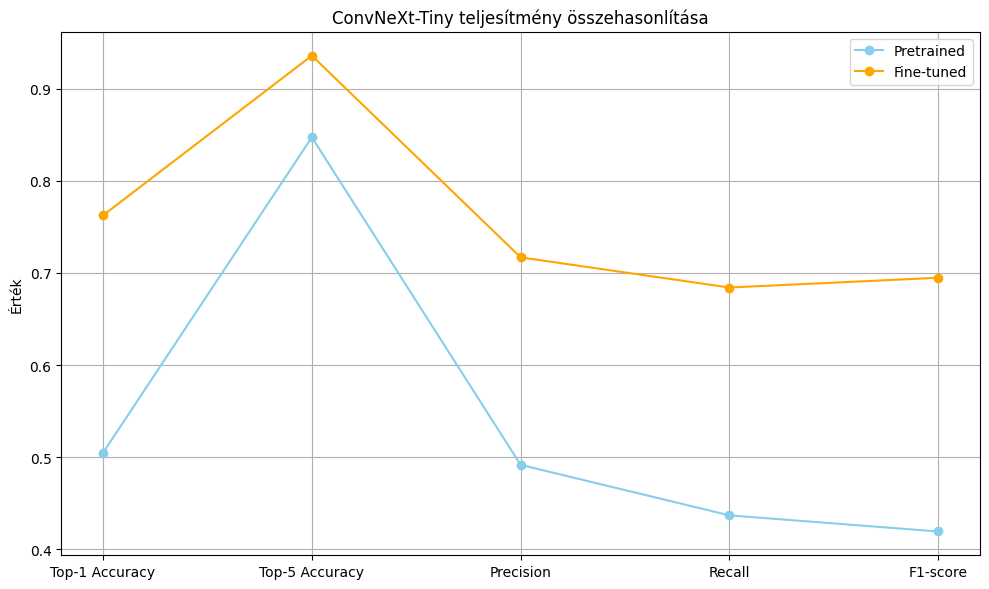
\includegraphics[width=1.0\textwidth]{images/phase02/ConvNeXt-Tiny_compare02.png}
      \caption{ConvNeXt-Tiny eredményeinek összehasonlítása}
      \label{fig:ConvNeXt-Tiny_compare02}
    \end{figure}

    \subsubsection{ConvNeXt-Tiny teljes tanítás utáni normalizált Confusion Mátrix}
    \begin{figure}[H]
      \centering
      
\includegraphics[width=0.8\textwidth]{images/phase02/ConvNeXt-Tiny_normalised_conf_mat.png}
      \caption{ConvNeXt-Tiny teljes tanítás utáni normalizált Confusion Mátrix}
      \label{fig:phase02_ConvNeXt-Tiny_normalised_conf_mat}
    \end{figure}
  
    \subsubsection{ConvNeXt-Tiny normalizált Confusion Mátrixok összehasonlítása}
    \begin{figure}[H]
      \centering
      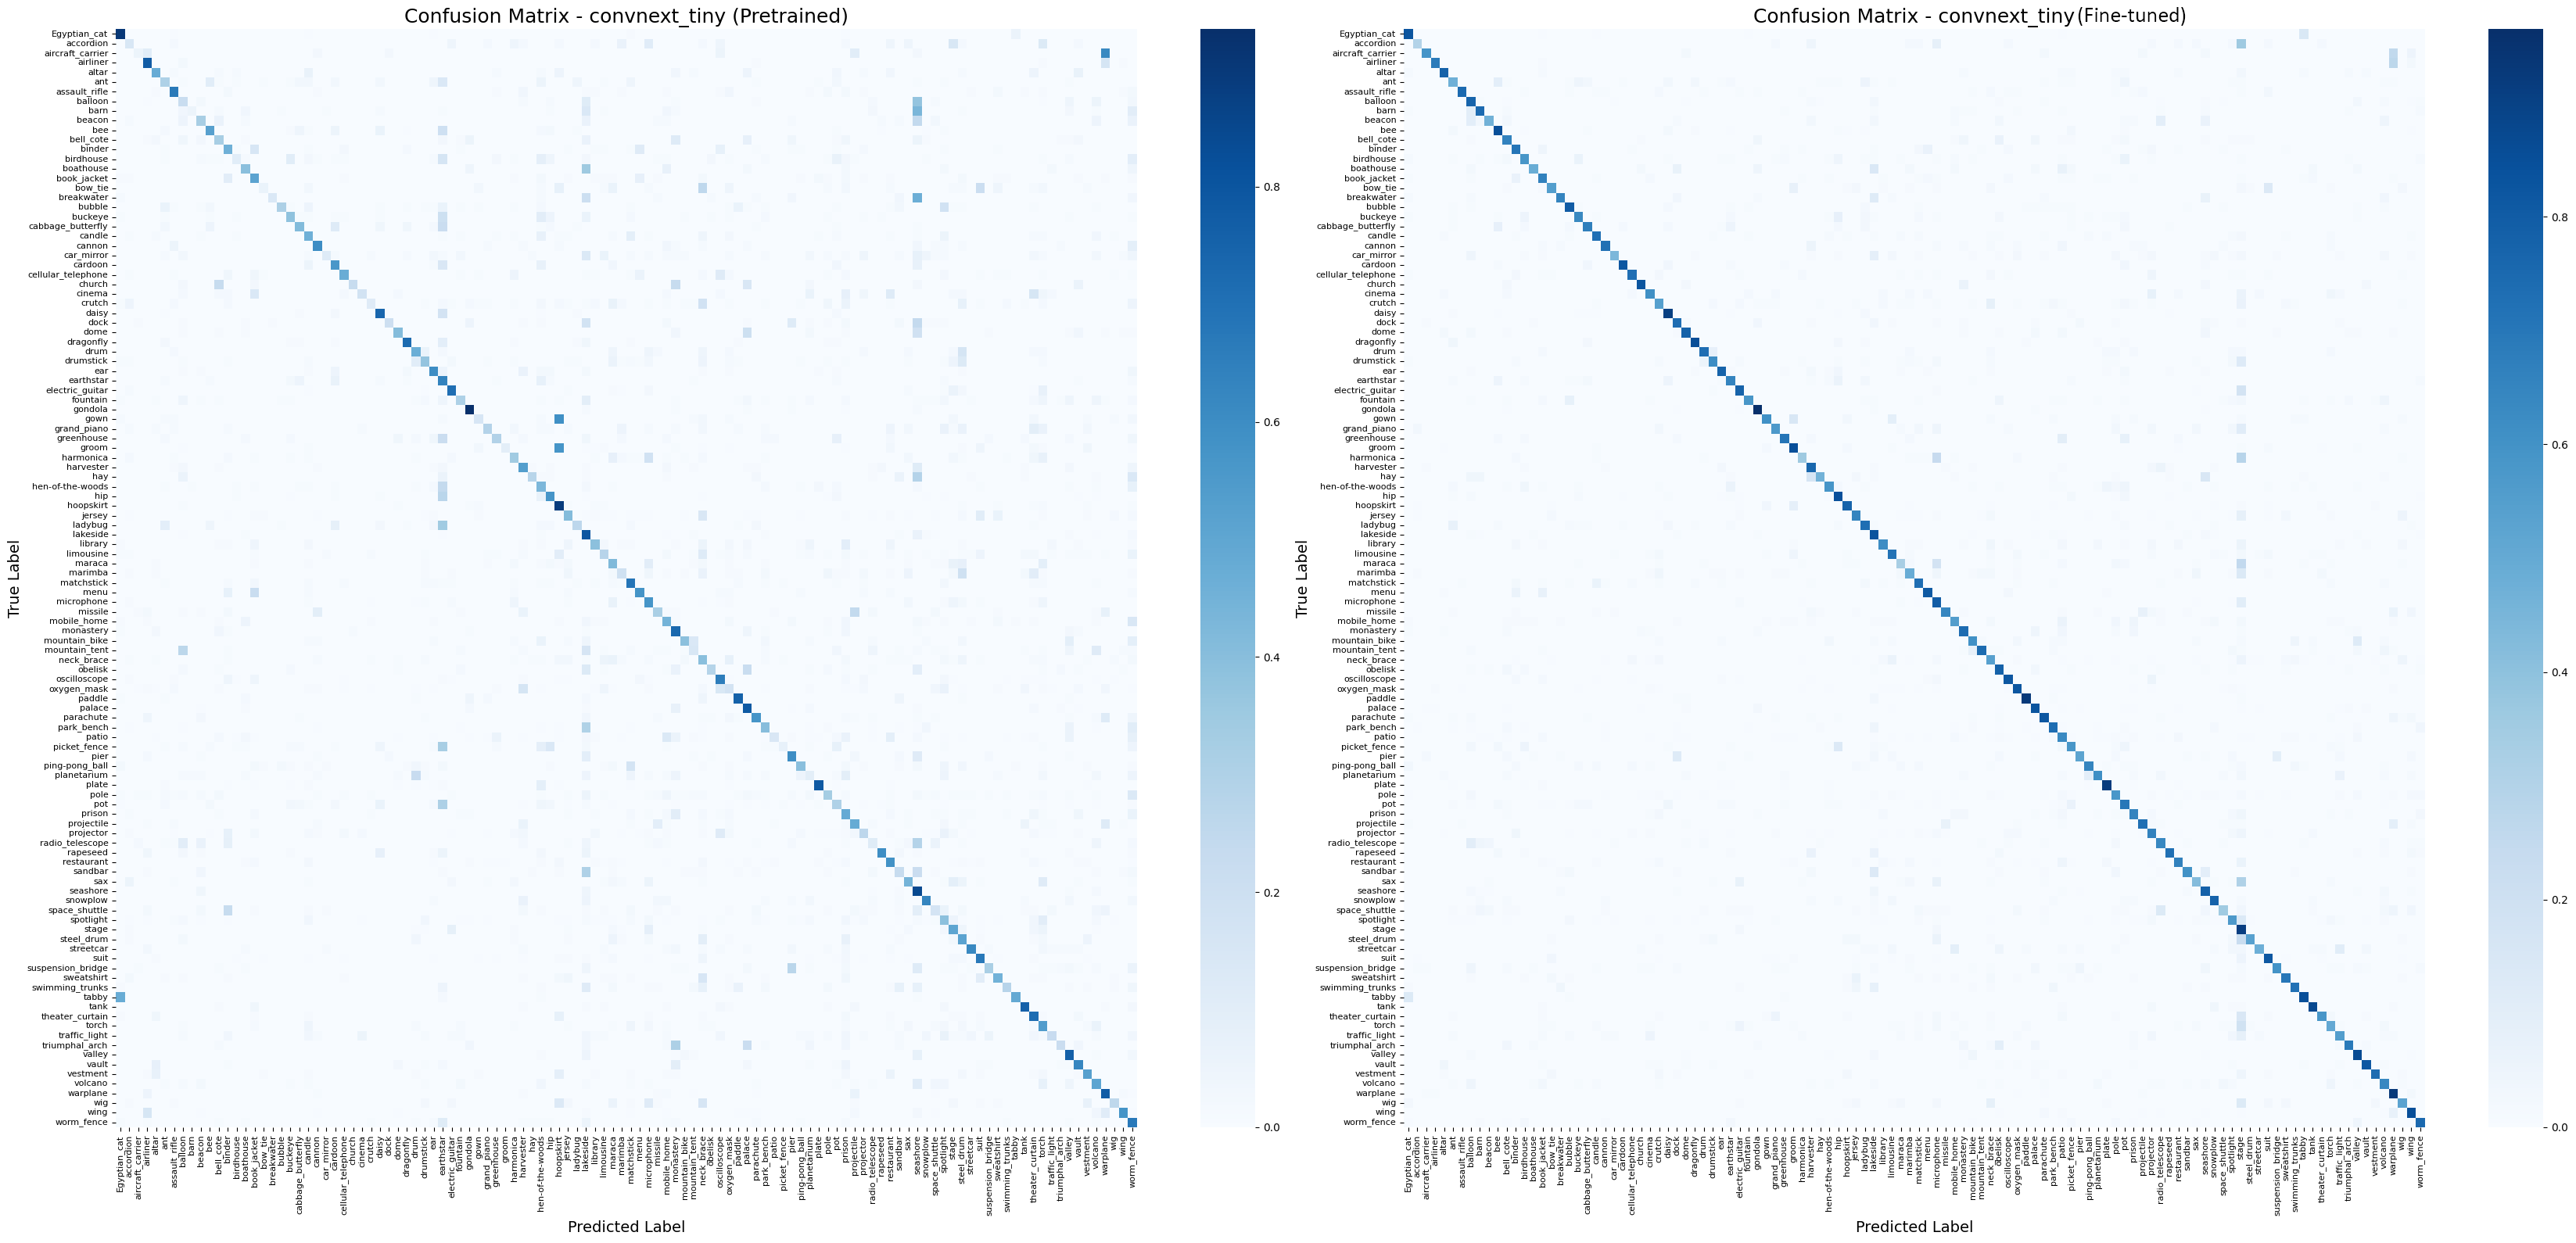
\includegraphics[width=1.0\textwidth]{images/phase02/ConvNeXt-Tiny_normalised_conf_mat_compare.png}
      \caption{ConvNeXt-Tiny normalizált Confusion Mátrixok összehasonlítása}
      \label{fig:phase02_ConvNeXt-Tiny_normalised_conf_mat_compare}
    \end{figure}


    \section{ViT-B/16}
    \subsubsection{ViT-B-16 teljes tanítás folyamata}
  \begin{figure}[H]
    \centering
    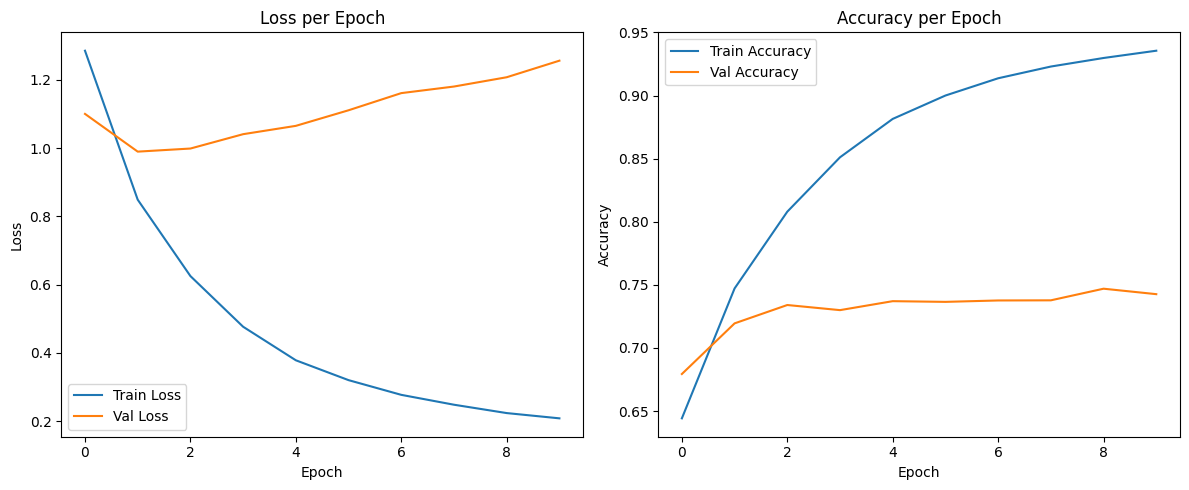
\includegraphics[width=1.0\textwidth]{images/phase02/ViT-B-16_learning_curve.png}
    \caption{ViT-B-16 teljes tanítás utáni sima Confusion Mátrix}
    \label{fig:phase02_ViT-B-16_learning_curves}
  \end{figure}

\subsubsection{ViT-B-16 teljes tanítás utáni eredményei}
  \begin{center}
  \begin{longtable}{l c}
  \caption{ViT-B-16 teljes tanítás utáni vizsgálati eredményei} \label{tab:phase02_ViT-B-16} \\
  \toprule
  \textbf{Metrika} & \textbf{Érték} \\
  \midrule
  \endfirsthead
  \toprule
  \textbf{Metrika} & \textbf{Érték} \\
  \midrule
  \endhead
  Top-1 Accuracy & 0.7414 \\
  Top-5 Accuracy & 0.9257 \\
  Precision & 0.6935 \\
  Recall & 0.6636 \\
  F1-score & 0.6730 \\
  Inference time & 42.40 sec \\
  \bottomrule
  \end{longtable}
  \end{center}

\subsubsection{ViT-B-16 eredményeinek összehasonlítása}
  \begin{center}
  \begin{longtable}{l c c}
  \caption{ViT-B-16 eredményeinek összehasonlítása} \label{tab:phase02_ViT-B-16_compare} \\
  \toprule
  \textbf{Metrika} & \textbf{Pretrained} & \textbf{Fine-tuned} \\
  \midrule
  \endfirsthead
  \toprule
  \textbf{Metrika} & \textbf{Pretrained} & \textbf{Fine-tuned} \\
  \midrule
  \endhead
  Top-1 Accuracy  & 0.5308 & 0.7414 \\
  Top-5 Accuracy & 0.8582 & 0.9257 \\
  Precision & 0.4629 & 0.6935 \\
  Recall & 0.4419 & 0.6636 \\
  F1-score & 0.4307 & 0.6908 \\
  Inference time & 92.13 sec & 42.40 sec \\
  \bottomrule
  \end{longtable}
  \end{center}

\subsubsection{ViT-B-16 eredményeinek összehasonlítása}
  \begin{figure}[H]
    \centering
    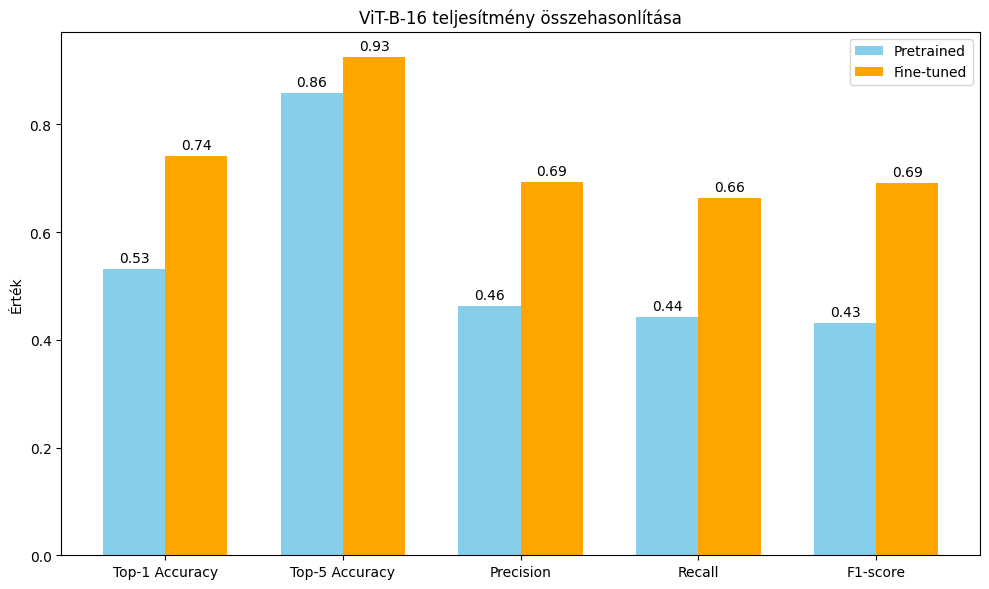
\includegraphics[width=1.0\textwidth]{images/phase02/ViT-B-16_compare01.png}
    \caption{ViT-B-16 eredményeinek összehasonlítása}
    \label{fig:ViT-B-16_compare01}
  \end{figure}

\subsubsection{ViT-B-16 eredményeinek összehasonlítása}
  \begin{figure}[H]
    \centering
    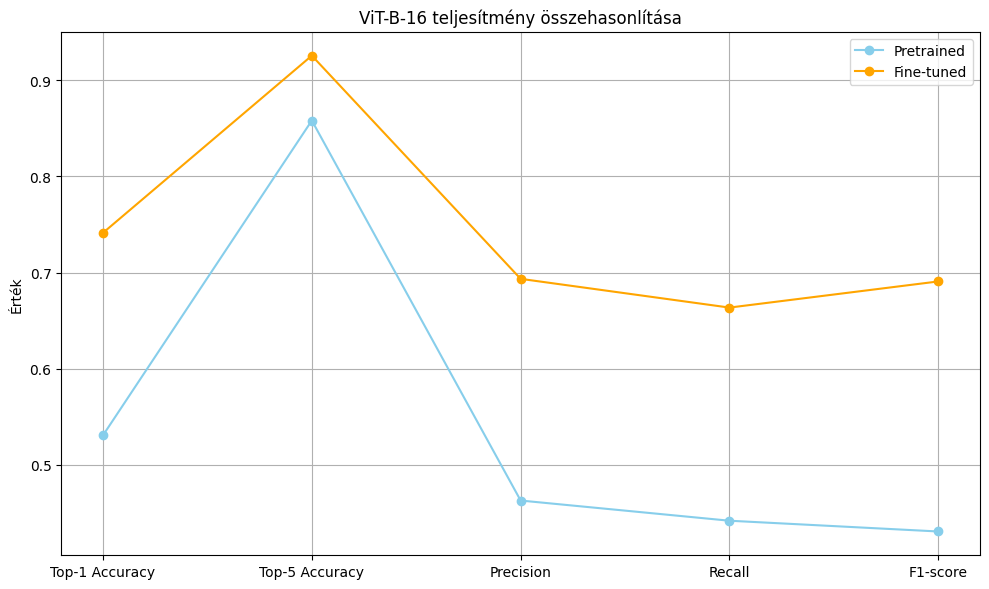
\includegraphics[width=1.0\textwidth]{images/phase02/ViT-B-16_compare02.png}
    \caption{ViT-B-16 eredményeinek összehasonlítása}
    \label{fig:ViT-B-16_compare02}
  \end{figure}

  \subsubsection{ViT-B-16 teljes tanítás utáni normalizált Confusion Mátrix}
  \begin{figure}[H]
    \centering
    
\includegraphics[width=0.8\textwidth]{images/phase02/ViT-B-16_normalised_conf_mat.png}
    \caption{ViT-B-16 teljes tanítás utáni normalizált Confusion Mátrix}
    \label{fig:phase02_ViT-B-16_normalised_conf_mat}
  \end{figure}

  \subsubsection{ViT-B-16 normalizált Confusion Mátrixok összehasonlítása}
  \begin{figure}[H]
    \centering
    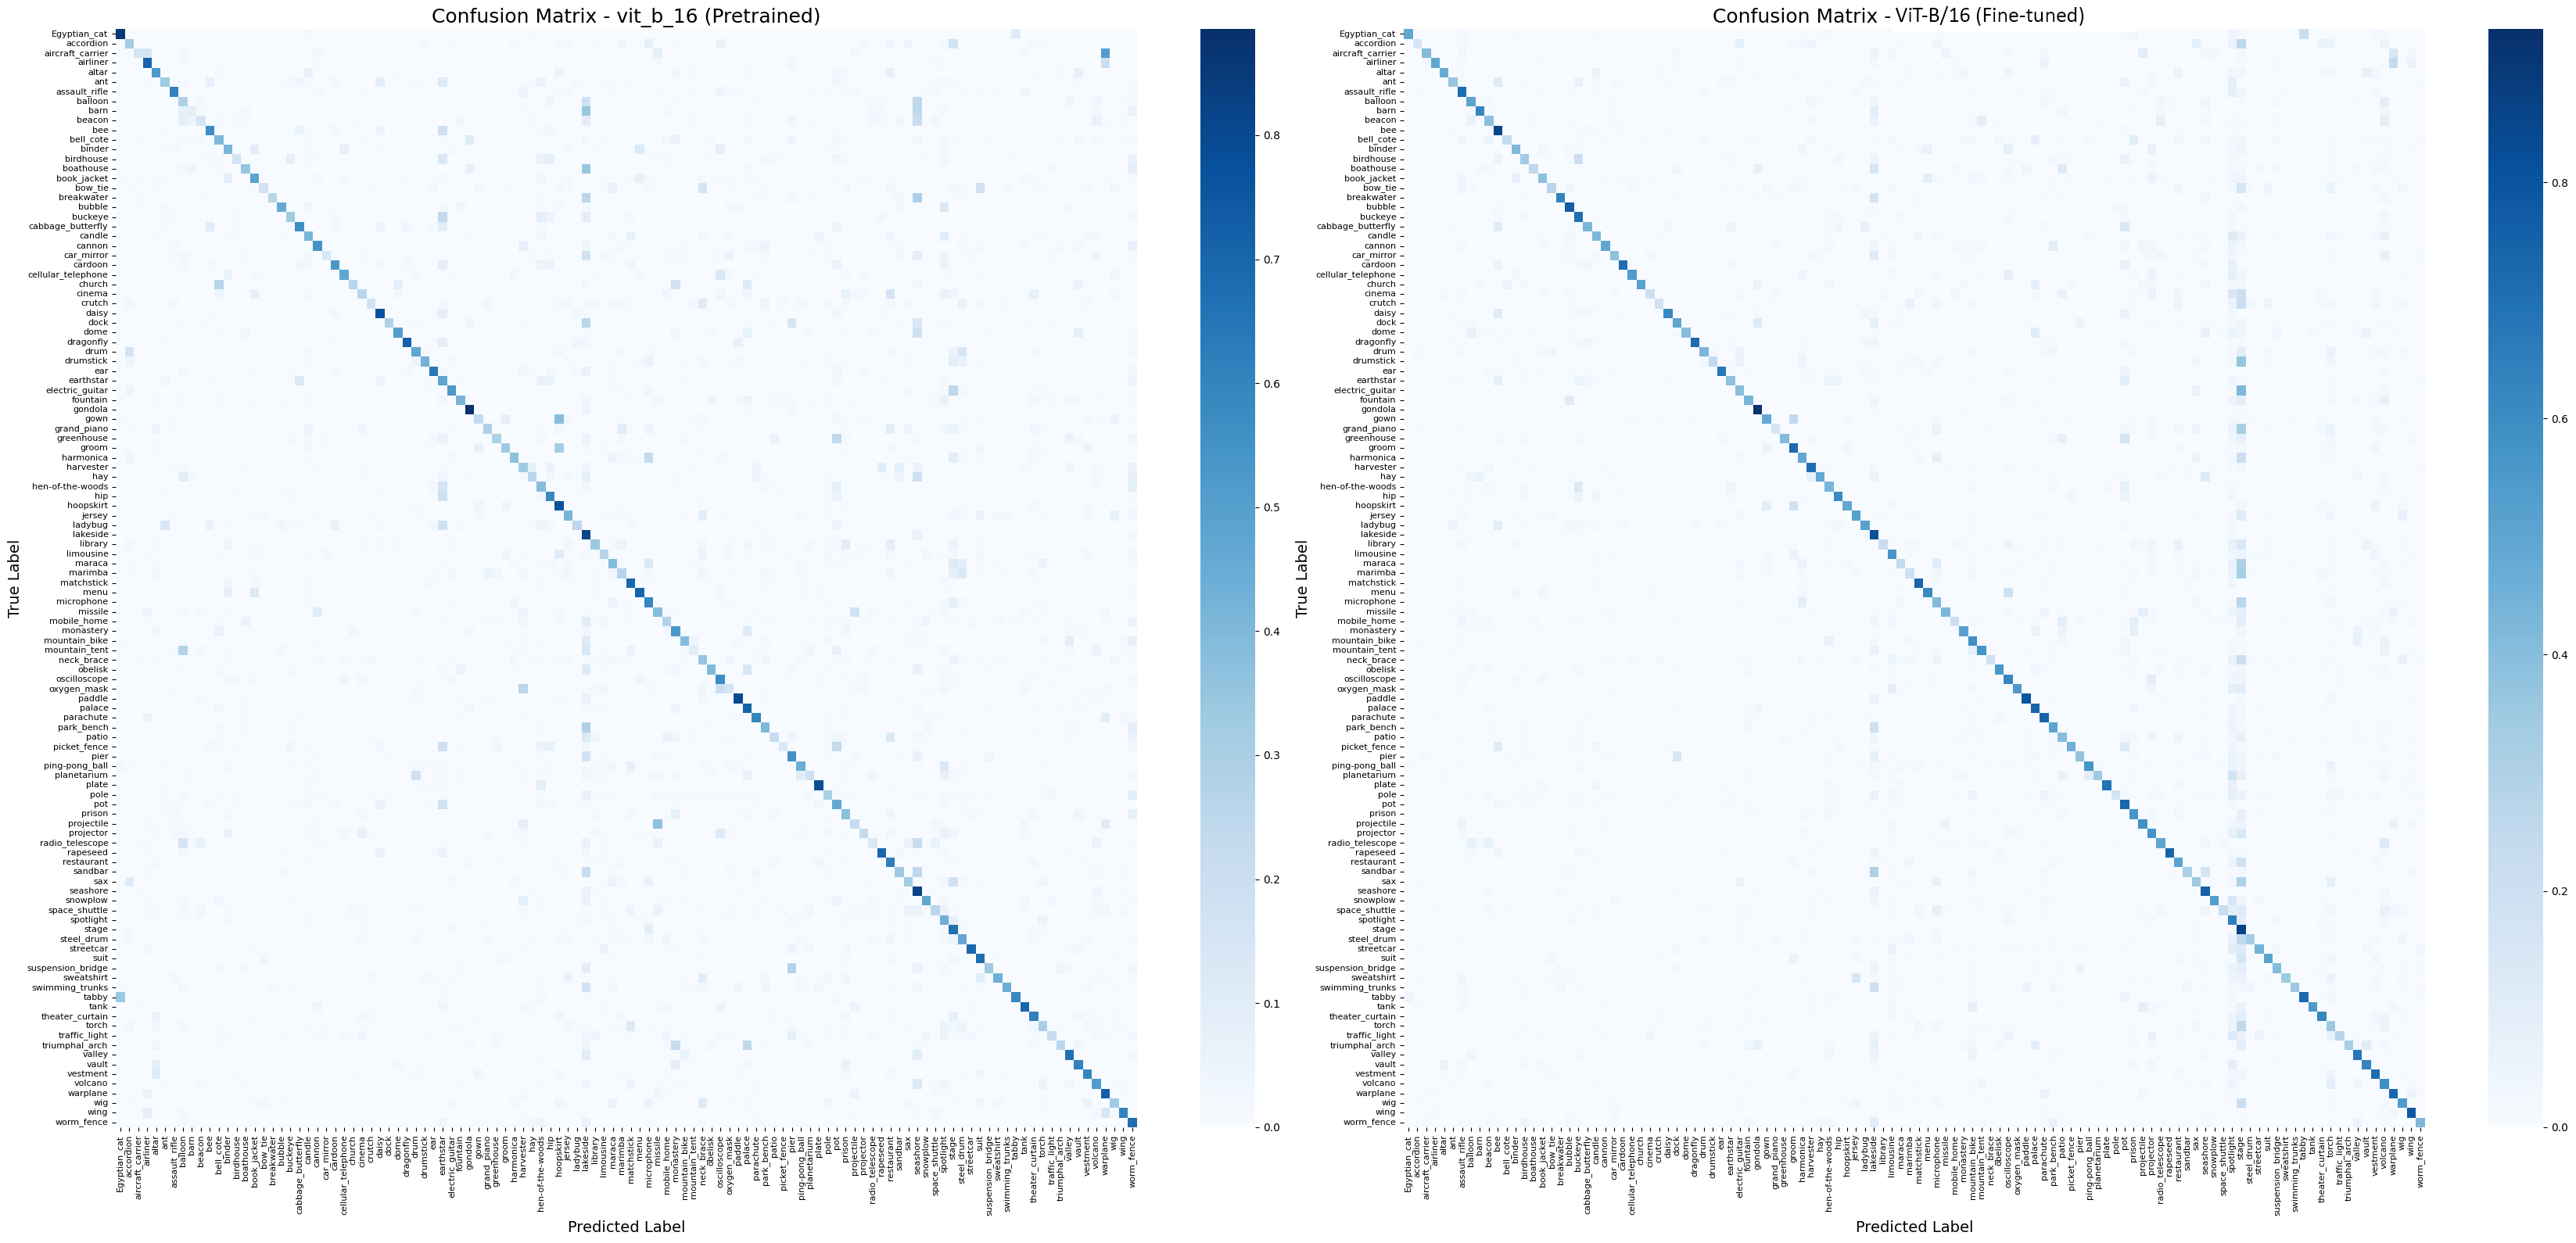
\includegraphics[width=1.0\textwidth]{images/phase02/ViT-B-16_normalised_conf_mat_compare.png}
    \caption{ViT-B-16 normalizált Confusion Mátrixok összehasonlítása}
    \label{fig:phase02_ViT-B-16_normalised_conf_mat_compare}
  \end{figure}


    \section{Inception-v3}
    \subsubsection{Inception-v3 teljes tanítás folyamata}
  \begin{figure}[H]
    \centering
    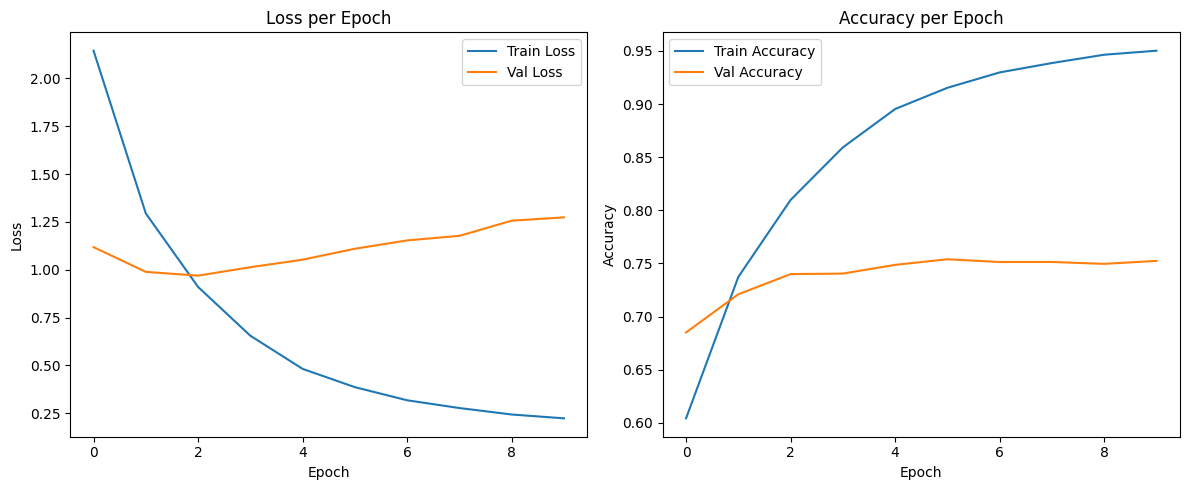
\includegraphics[width=1.0\textwidth]{images/phase02/Inception-v3_learning_curve.png}
    \caption{Inception-v3 teljes tanítás utáni sima Confusion Mátrix}
    \label{fig:phase02_Inception-v3_learning_curves}
  \end{figure}

\subsubsection{Inception-v3 teljes tanítás utáni eredményei}
  \begin{center}
  \begin{longtable}{l c}
  \caption{Inception-v3 teljes tanítás utáni vizsgálati eredményei} \label{tab:phase02_Inception-v3} \\
  \toprule
  \textbf{Metrika} & \textbf{Érték} \\
  \midrule
  \endfirsthead
  \toprule
  \textbf{Metrika} & \textbf{Érték} \\
  \midrule
  \endhead
  Top-1 Accuracy & 0.7518 \\
  Top-5 Accuracy & 0.9320 \\
  Precision & 0.6963 \\
  Recall & 0.6787 \\
  F1-score & 0.6908 \\
  Inference time & 25.11 sec \\
  \bottomrule
  \end{longtable}
  \end{center}

\subsubsection{Inception-v3 eredményeinek összehasonlítása}
  \begin{center}
  \begin{longtable}{l c c}
  \caption{Inception-v3 eredményeinek összehasonlítása} \label{tab:phase02_Inception-v3_compare} \\
  \toprule
  \textbf{Metrika} & \textbf{Pretrained} & \textbf{Fine-tuned} \\
  \midrule
  \endfirsthead
  \toprule
  \textbf{Metrika} & \textbf{Pretrained} & \textbf{Fine-tuned} \\
  \midrule
  \endhead
  Top-1 Accuracy  & 0.4763 & 0.7518 \\
  Top-5 Accuracy & 0.8008 & 0.9320 \\
  Precision & 0.3833 & 0.6963 \\
  Recall & 0.3896 & 0.6787 \\
  F1-score & 0.3683 & 0.6827 \\
  Inference time & 38.06 sec & 33.62 sec \\
  \bottomrule
  \end{longtable}
  \end{center}

\subsubsection{Inception-v3 eredményeinek összehasonlítása}
  \begin{figure}[H]
    \centering
    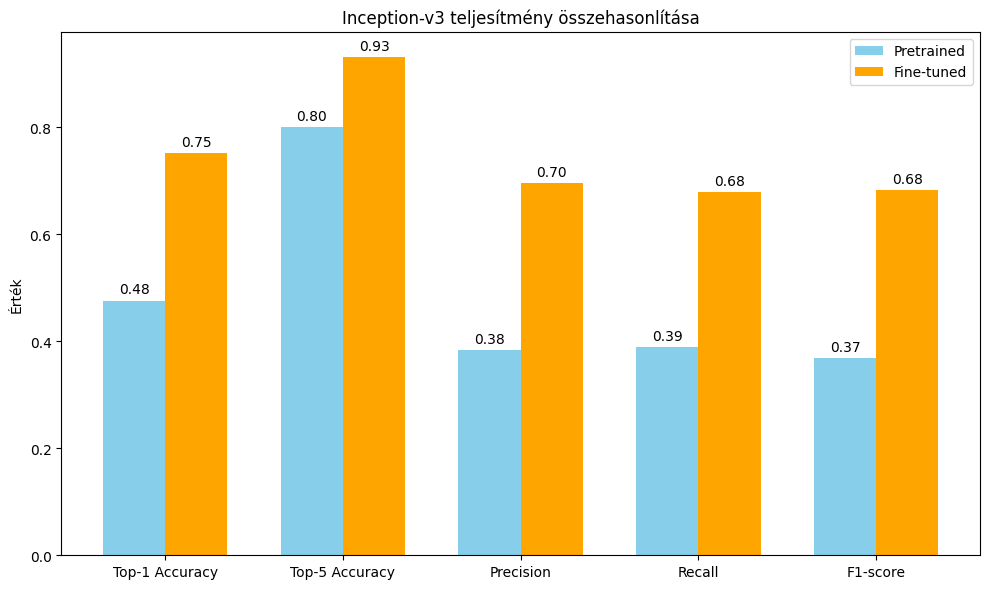
\includegraphics[width=1.0\textwidth]{images/phase02/Inception-v3_compare01.png}
    \caption{Inception-v3 eredményeinek összehasonlítása}
    \label{fig:Inception-v3_compare01}
  \end{figure}

\subsubsection{Inception-v3 eredményeinek összehasonlítása}
  \begin{figure}[H]
    \centering
    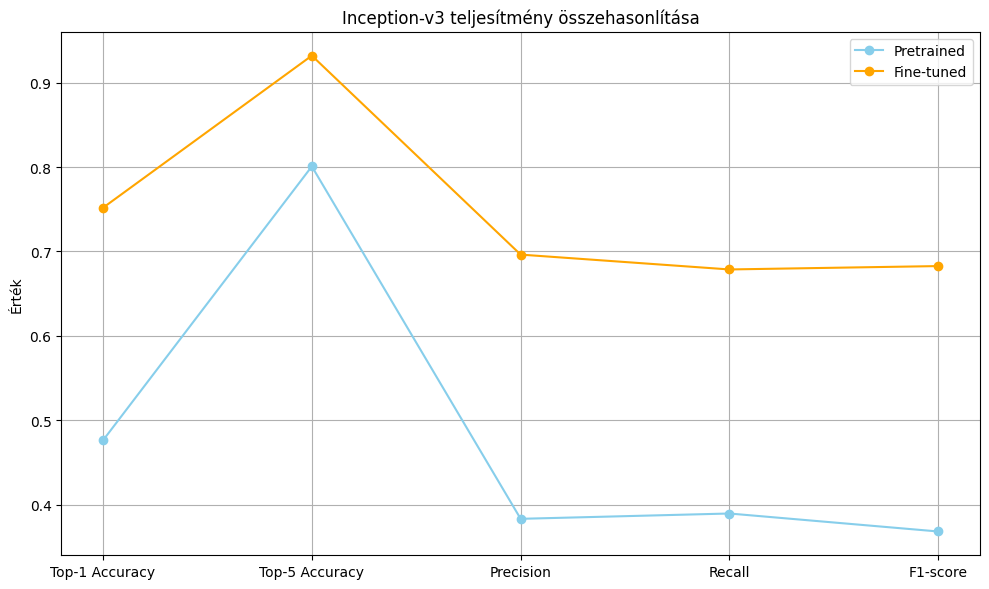
\includegraphics[width=1.0\textwidth]{images/phase02/Inception-v3_compare02.png}
    \caption{Inception-v3 eredményeinek összehasonlítása}
    \label{fig:Inception-v3_compare02}
  \end{figure}

  \subsubsection{Inception-v3 teljes tanítás utáni normalizált Confusion Mátrix}
  \begin{figure}[H]
    \centering
    
\includegraphics[width=0.8\textwidth]{images/phase02/Inception-v3_normalised_conf_mat.png}
    \caption{Inception-v3 teljes tanítás utáni normalizált Confusion Mátrix}
    \label{fig:phase02_Inception-v3_normalised_conf_mat}
  \end{figure}

  \subsubsection{Inception-v3 normalizált Confusion Mátrixok összehasonlítása}
  \begin{figure}[H]
    \centering
    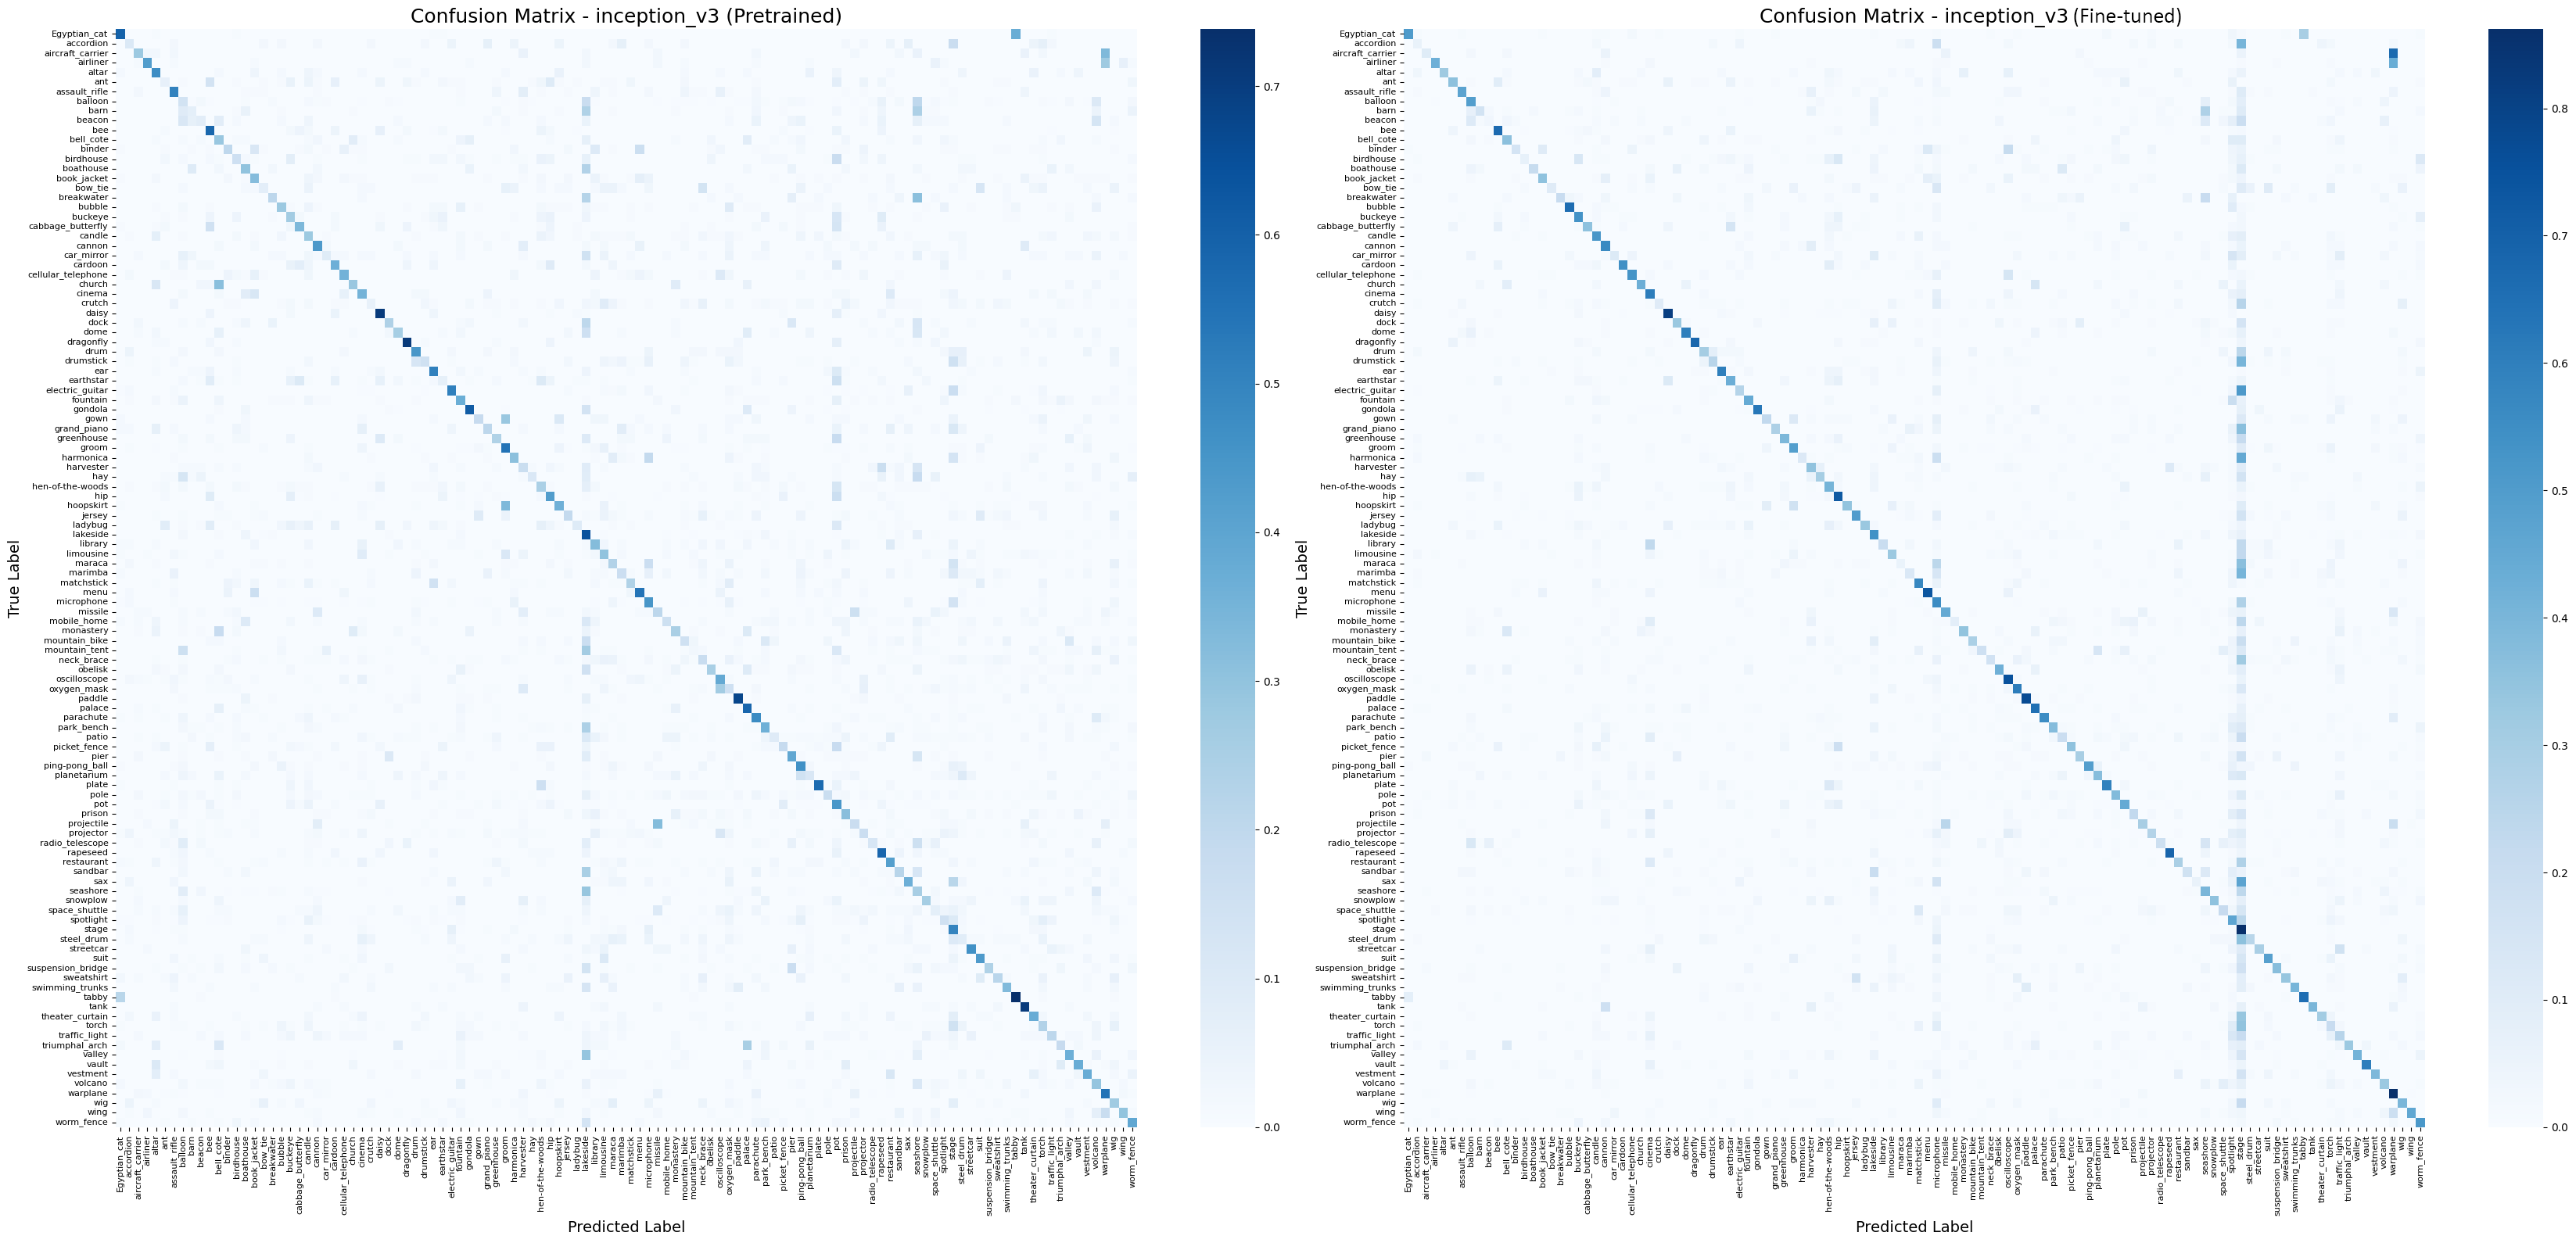
\includegraphics[width=1.0\textwidth]{images/phase02/Inception-v3_normalised_conf_mat_compare.png}
    \caption{Inception-v3 normalizált Confusion Mátrixok összehasonlítása}
    \label{fig:phase02_Inception-v3_normalised_conf_mat_compare}
  \end{figure}


    \section{NASNet}
    \subsubsection{NASNet teljes tanítás folyamata}
  \begin{figure}[H]
    \centering
    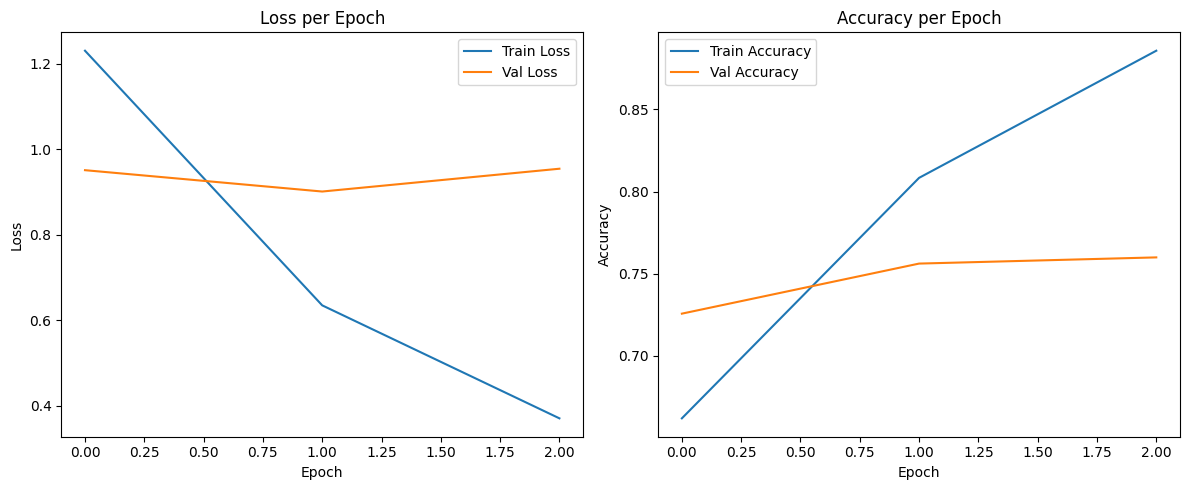
\includegraphics[width=1.0\textwidth]{images/phase02/NASNet_learning_curve.png}
    \caption{NASNet teljes tanítás utáni sima Confusion Mátrix}
    \label{fig:phase02_NASNet_learning_curves}
  \end{figure}

\subsubsection{NASNet teljes tanítás utáni eredményei}
  \begin{center}
  \begin{longtable}{l c}
  \caption{NASNet teljes tanítás utáni vizsgálati eredményei} \label{tab:phase02_NASNet} \\
  \toprule
  \textbf{Metrika} & \textbf{Érték} \\
  \midrule
  \endfirsthead
  \toprule
  \textbf{Metrika} & \textbf{Érték} \\
  \midrule
  \endhead
  Top-1 Accuracy & 0.7626 \\
  Top-5 Accuracy & 0.9470 \\
  Precision & 0.7180 \\
  Recall & 0.6875 \\
  F1-score & 0.6955 \\
  Inference time & 25.11 sec \\
  \bottomrule
  \end{longtable}
  \end{center}

\subsubsection{NASNet eredményeinek összehasonlítása}
  \begin{center}
  \begin{longtable}{l c c}
  \caption{NASNet eredményeinek összehasonlítása} \label{tab:phase02_NASNet_compare} \\
  \toprule
  \textbf{Metrika} & \textbf{Pretrained} & \textbf{Fine-tuned} \\
  \midrule
  \endfirsthead
  \toprule
  \textbf{Metrika} & \textbf{Pretrained} & \textbf{Fine-tuned} \\
  \midrule
  \endhead
  Top-1 Accuracy  & 0.2820 & 0.7626 \\
  Top-5 Accuracy & 0.5408 & 0.9470 \\
  Precision & 0.3204 & 0.7180 \\
  Recall & 0.2799 & 0.6808 \\
  F1-score & 0.2696 & 0.6955 \\
  Inference time & 275.30 sec & 34.03 sec \\
  \bottomrule
  \end{longtable}
  \end{center}

\subsubsection{NASNet eredményeinek összehasonlítása}
  \begin{figure}[H]
    \centering
    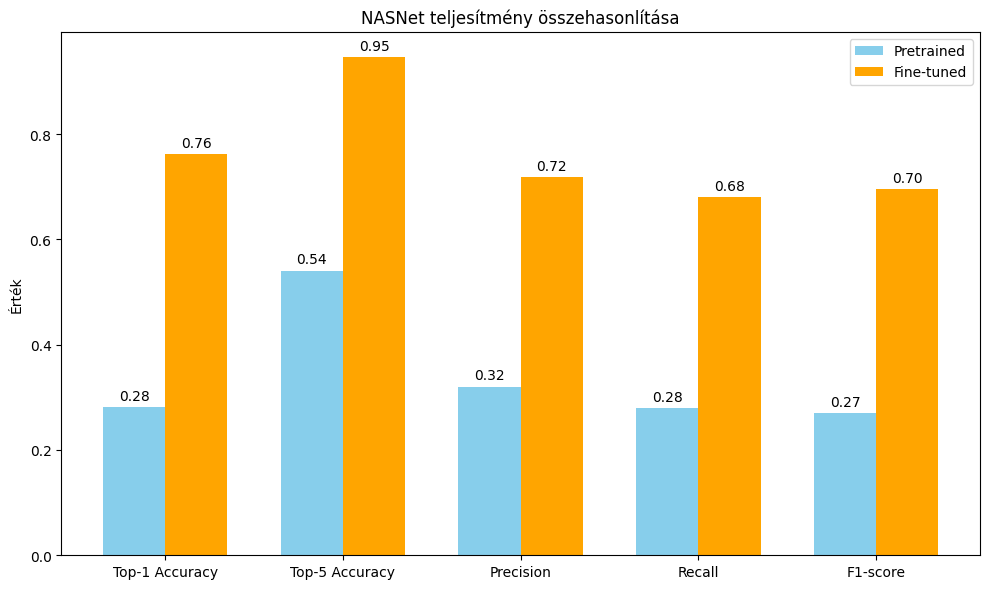
\includegraphics[width=1.0\textwidth]{images/phase02/NASNet_compare01.png}
    \caption{NASNet eredményeinek összehasonlítása}
    \label{fig:NASNet_compare01}
  \end{figure}

\subsubsection{NASNet eredményeinek összehasonlítása}
  \begin{figure}[H]
    \centering
    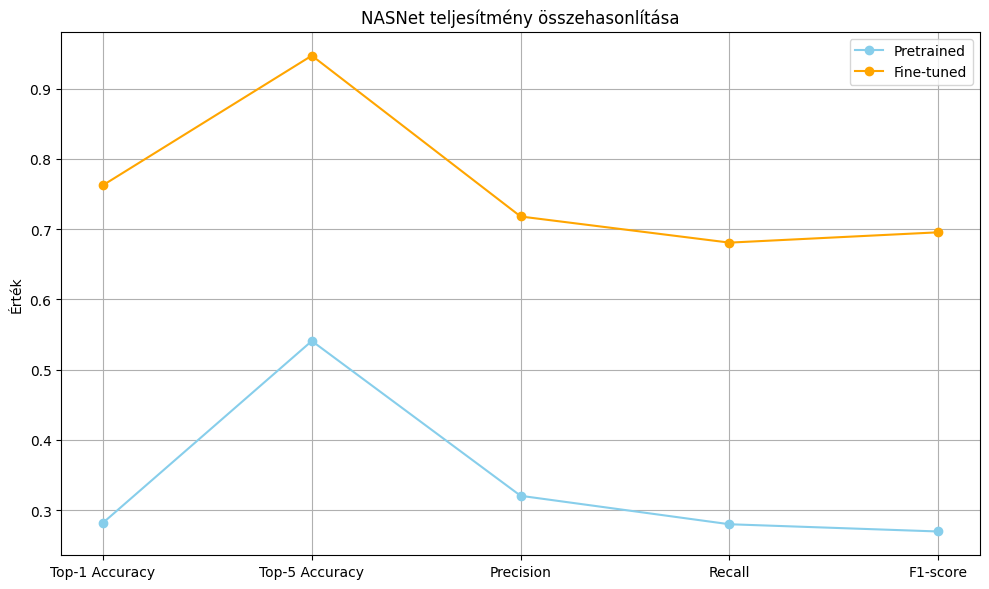
\includegraphics[width=1.0\textwidth]{images/phase02/NASNet_compare02.png}
    \caption{NASNet eredményeinek összehasonlítása}
    \label{fig:NASNet_compare02}
  \end{figure}

  \subsubsection{NASNet teljes tanítás utáni normalizált Confusion Mátrix}
  \begin{figure}[H]
    \centering
    
\includegraphics[width=0.8\textwidth]{images/phase02/NASNet_normalised_conf_mat.png}
    \caption{NASNet teljes tanítás utáni normalizált Confusion Mátrix}
    \label{fig:phase02_NASNet_normalised_conf_mat}
  \end{figure}

  \subsubsection{NASNet normalizált Confusion Mátrixok összehasonlítása}
  \begin{figure}[H]
    \centering
    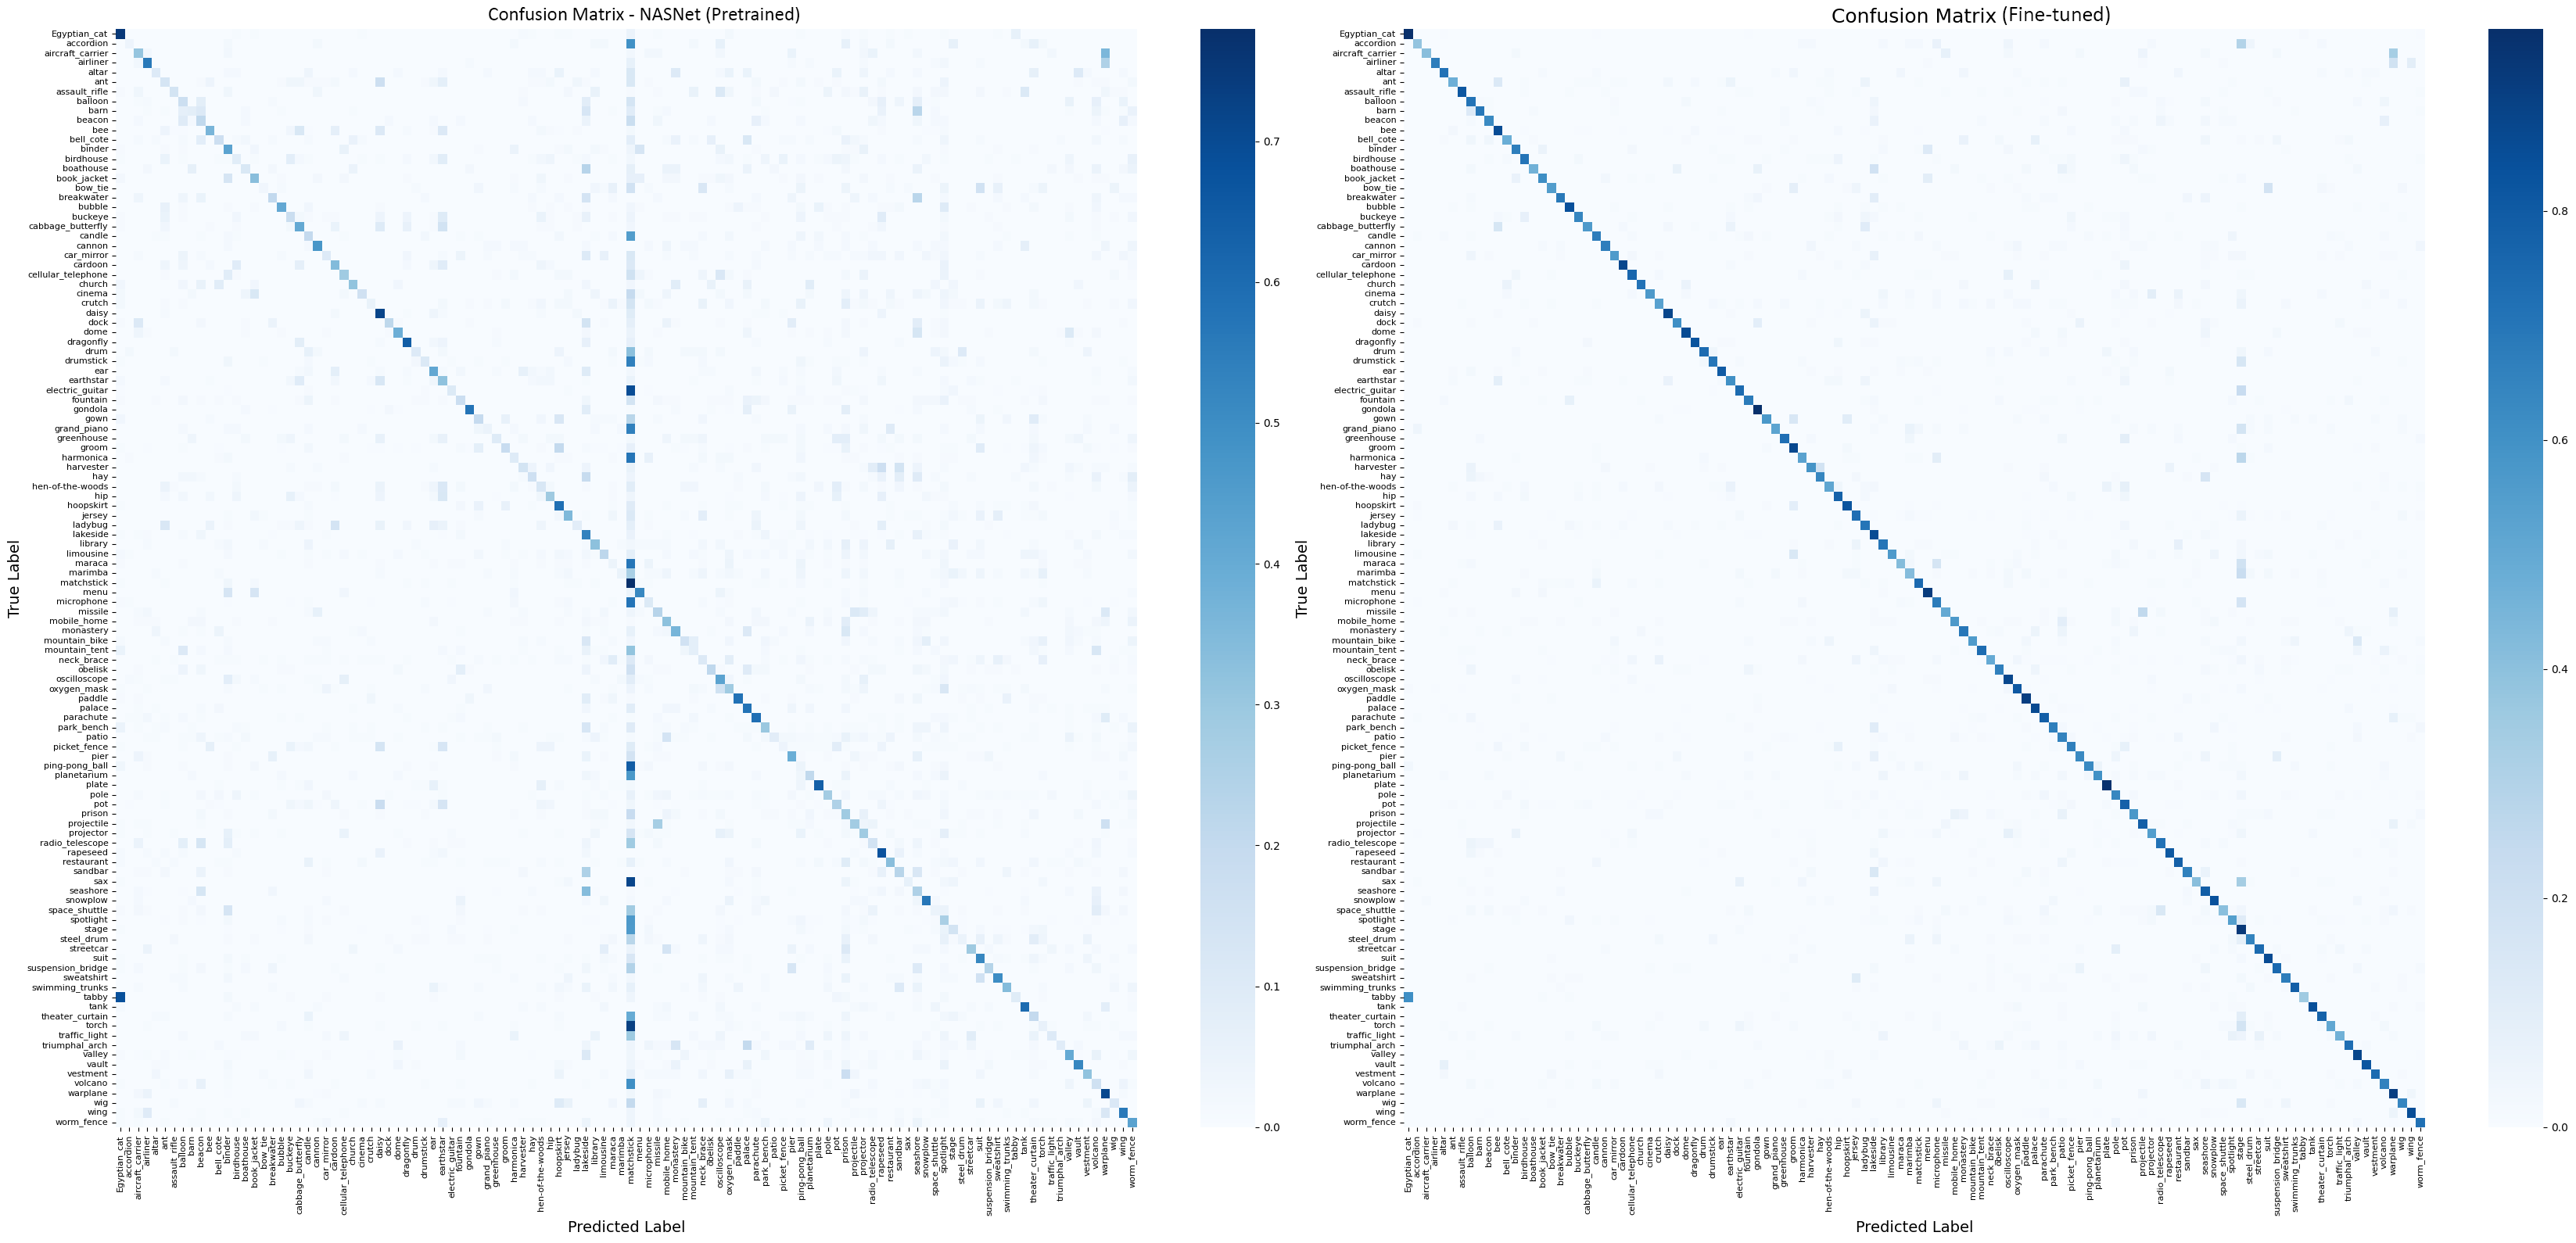
\includegraphics[width=1.0\textwidth]{images/phase02/NASNet_normalised_conf_mat_compare.png}
    \caption{NASNet normalizált Confusion Mátrixok összehasonlítása}
    \label{fig:phase02_NASNet_normalised_conf_mat_compare}
  \end{figure}


\section{Összefoglaló}

Ebben a fázisban a hét ismert modellt teszteltem úgy, hogy a 180750 képből álló sb-photothemes180k ImageNet1k cimkék szerint címkézett adathalmazon tanítottam, ahol 114 kategória van ebben a második vizsgálati fázisban a 144000 kategorizált tanító és 18000 validáló kép segítségével végeztem teljes tanítást 10 epoch-on keresztül, majd a 18000 képet tartalmazó teszt halmazon teszteltem le a modelleket ugyanazon amin az első fázisban a tanítás nélküli teszteket is végeztem. 

\subsection{Összefoglaló táblázat a második fázis mért értékeiről.}
    \begin{center}
        \begin{longtable}{lllllll}
        \caption{Összefoglaló táblázat a második fázis mért értékeiről}\label{tab:phase2_summary_table_01}\\
        \toprule
        Modell & Top-1 & Top-5 & Precision & Recall & F1 & Time(s) \\
        \midrule
        \endfirsthead
        \toprule
        Modell & Top-1 & Top-5 & Precision & Recall & F1 & Time(s) \\
        \midrule
        \endhead
        NASNet & 0.7626 & 0.9470 & 0.7180 & 0.6875 & 0.6955 & 25.11 \\
        ConvNeXt-Tiny & 0.7624 & 0.9357 & 0.7168 & 0.6841 & 0.6947 & 25.67 \\
        EfficientNet-B0 & 0.7649 & 0.9421 & 0.7130 & 0.6950 & 0.7001 & 25.26 \\
        ResNet50 & 0.7553 & 0.9351 & 0.7110 & 0.6808 & 0.6908 & 25.11 \\
        Inception-v3 & 0.7518 & 0.9320 & 0.6963 & 0.6787 & 0.6908 & 25.11 \\
        ViT-B/16 & 0.7414 & 0.9257 & 0.6935 & 0.6636 & 0.6730 & 42.40 \\
        DenseNet121 & 0.7400 & 0.9266 & 0.6811 & 0.6808 & 0.6696 & 25.23 \\
        \bottomrule
        \end{longtable}
    \end{center}

\subsection{Top 1 pontosságok összehasonlítása teljes tanítás után.}
    \begin{figure}[H]
        \centering
        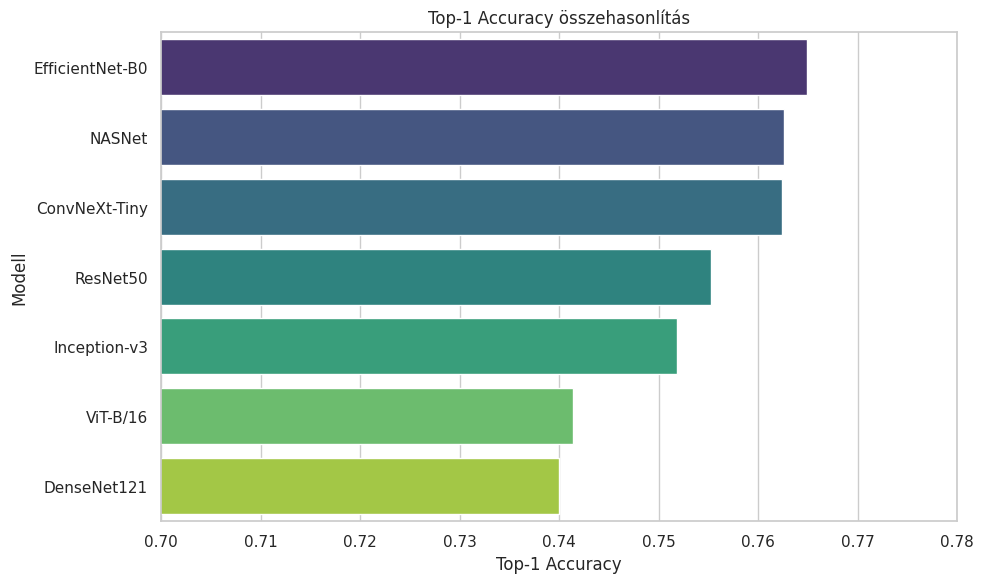
\includegraphics[width=1.0\textwidth]{images/phase02/phase02_summary_top1.png}
        \caption{Top 1 pontosságok összehasonlítása teljes tanítás után.}
        \label{fig:phase02_summary_top1}
    \end{figure}

\subsection{F1 értékek összehasonlítása teljes tanítás után.}
    \begin{figure}[H]
        \centering
        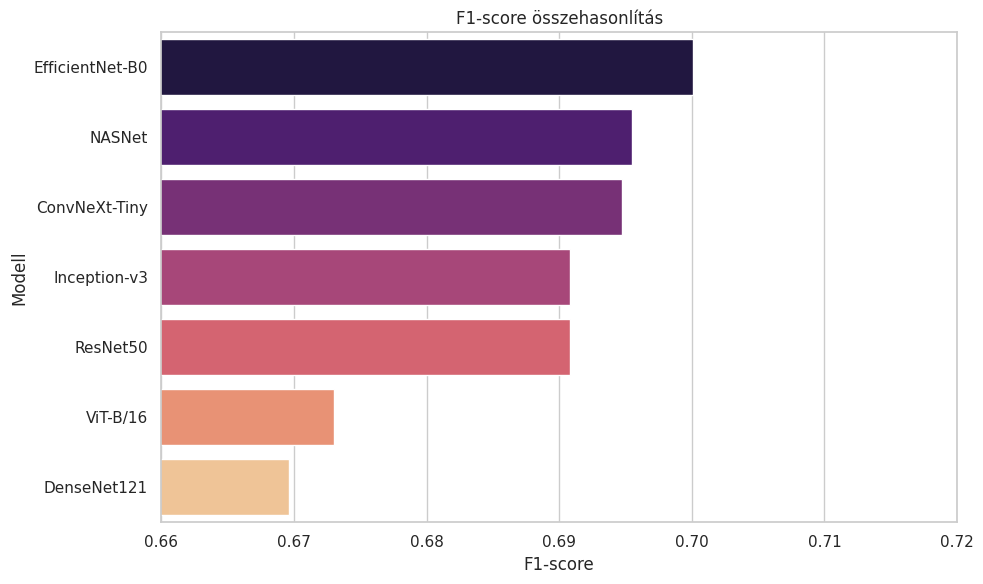
\includegraphics[width=1.0\textwidth]{images/phase02/phase02_summary_f1.png}
        \caption{F1 értékek összehasonlítása teljes tanítás után.}
        \label{fig:phase02_summary_top1}
    \end{figure}

\subsection{Futási idők összehasonlítása teljes tanítás után a teszt halmazon.}
    \begin{figure}[H]
        \centering
        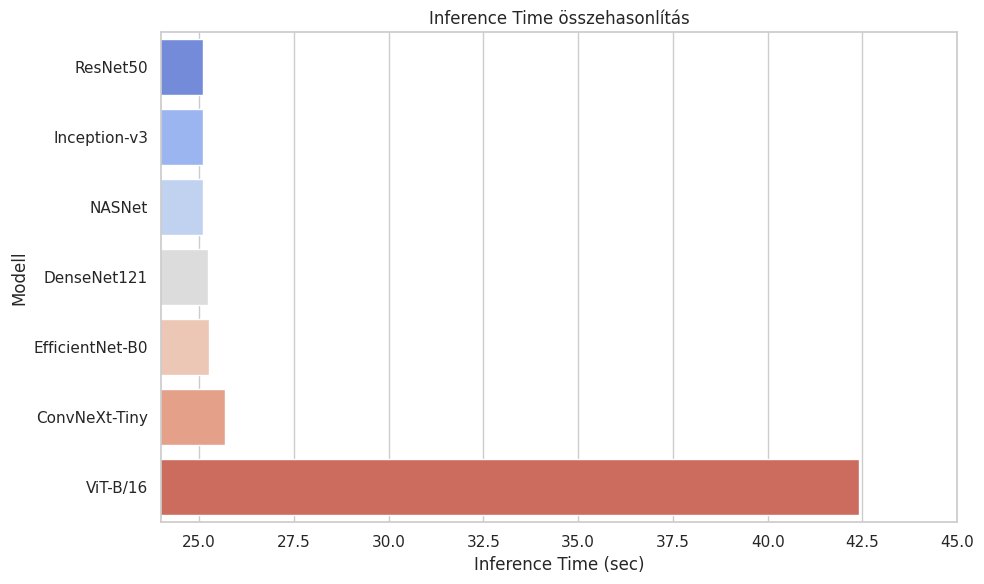
\includegraphics[width=1.0\textwidth]{images/phase02/phase02_summary_time.png}
        \caption{Futási idők összehasonlítása teljes tanítás után a teszt halmazon.}
        \label{fig:phase02_summary_time}
    \end{figure}

\subsection{Top 1 és Top 5 pontosságok összehasonlítása teljes tanítás után a teszt halmazon.}
    \begin{figure}[H]
        \centering
        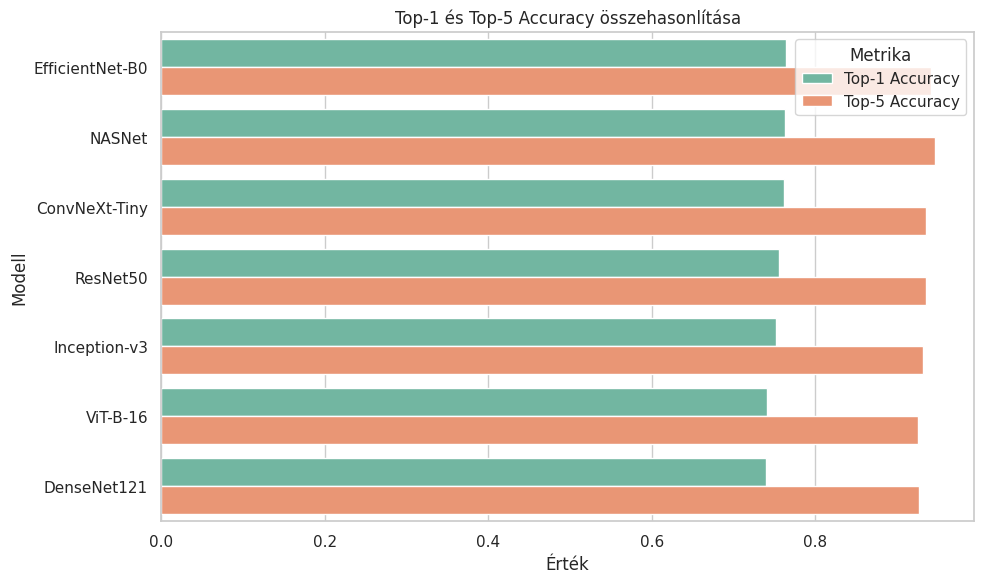
\includegraphics[width=1.0\textwidth]{images/phase02/phase02_summary_top1vstop5.png}
        \caption{Top 1 és Top 5 pontosságok összehasonlítása teljes tanítás után a teszt halmazon.}
        \label{fig:phase02_summary_top1vstop5}
    \end{figure}

\subsection{Precision, Recall és F1 összehasonlítása teljes tanítás után a teszt halmazon.}
    \begin{figure}[H]
        \centering
        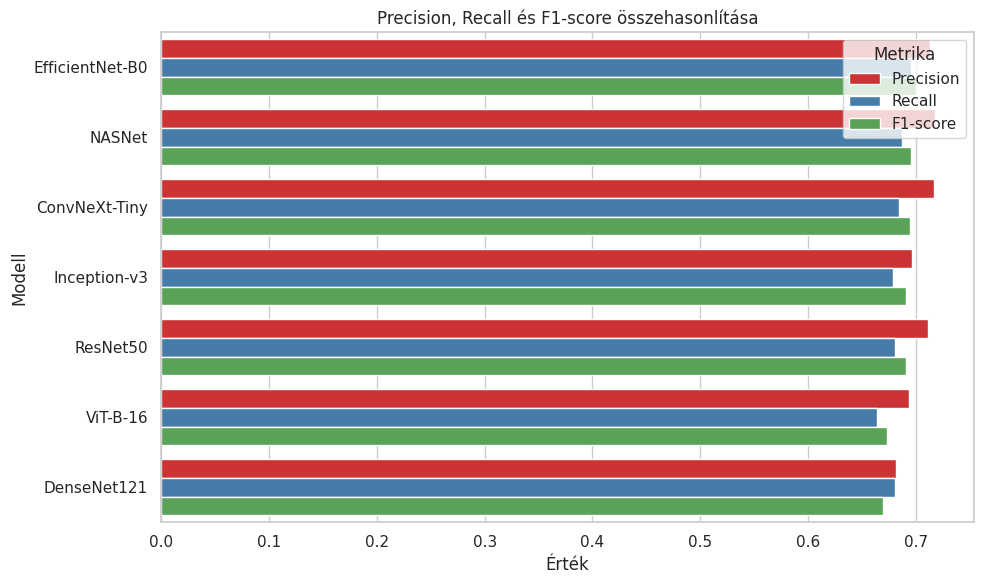
\includegraphics[width=1.0\textwidth]{images/phase02/phase02_summary_prec_rec_f1.png}
        \caption{Precision, Recall és F1 összehasonlítása teljes tanítás után a teszt halmazon.}
        \label{fig:phase02_summary_prec_rec_f1}
    \end{figure}

\subsection{Összehasonlító táblázat az első és a második fázis mért értékeiről.}
    \begin{center}
        \begin{longtable}{lllll}
        \caption{Összehasonlító táblázat az első és a második fázis mért értékeiről – Alapvető metrikák}\label{tab:phase2_summary_table_02_basic}\\
        \toprule
        Modell & Top-1 (PT) & Top-1 (FT) & Top-5 (PT) & Top-5 (FT) \\
        \midrule
        \endfirsthead
        \toprule
        Modell & Top-1 (PT) & Top-1 (FT) & Top-5 (PT) & Top-5 (FT) \\
        \midrule
        \endhead
        ConvNeXt-Tiny & 0.5048 & 0.7624 & 0.8471 & 0.9357 \\
        EfficientNet-B0 & 0.4802 & 0.7649 & 0.8217 & 0.9421 \\
        ResNet50 & 0.4698 & 0.7553 & 0.7962 & 0.9351 \\
        Inception-v3 & 0.4763 & 0.7518 & 0.8008 & 0.9320 \\
        ViT-B-16 & 0.5308 & 0.7414 & 0.8582 & 0.9257 \\
        DenseNet121 & 0.4498 & 0.7400 & 0.7806 & 0.9266 \\
        \bottomrule
        \end{longtable}
    \end{center}
    

    \begin{center}
        \begin{longtable}{lllll}
        \caption{Összehasonlító táblázat az első és a második fázis mért értékeiről – Pontosság és visszahívás}\label{tab:phase2_summary_table_02_precision_recall}\\
        \toprule
        Modell & Precision (PT) & Precision (FT) & Recall (PT) & Recall (FT) \\
        \midrule
        \endfirsthead
        \toprule
        Modell & Precision (PT) & Precision (FT) & Recall (PT) & Recall (FT) \\
        \midrule
        \endhead
        ConvNeXt-Tiny & 0.4917 & 0.7168 & 0.4369 & 0.6841 \\
        EfficientNet-B0 & 0.4137 & 0.7130 & 0.4039 & 0.6950 \\
        ResNet50 & 0.3934 & 0.7110 & 0.3797 & 0.6808 \\
        Inception-v3 & 0.3833 & 0.6963 & 0.3896 & 0.6787 \\
        ViT-B-16 & 0.4629 & 0.6935 & 0.4419 & 0.6636 \\
        DenseNet121 & 0.3874 & 0.6811 & 0.3611 & 0.6680 \\
        \bottomrule
        \end{longtable}
    \end{center}
        

    \begin{center}
        \begin{longtable}{lllll}
        \caption{Összehasonlító táblázat az első és a második fázis mért értékeiről – F1 és idő}\label{tab:phase2_summary_table_02_f1_time}\\
        \toprule
        Modell & F1 (PT) & F1 (FT) & Time (PT) & Time (FT) \\
        \midrule
        \endfirsthead
        \toprule
        Modell & F1 (PT) & F1 (FT) & Time (PT) & Time (FT) \\
        \midrule
        \endhead
        ConvNeXt-Tiny & 0.4194 & 0.6947 & 38.40s & 25.67s \\
        EfficientNet-B0 & 0.3829 & 0.7001 & 28.89s & 25.26s \\
        ResNet50 & 0.3592 & 0.6908 & 25.21s & 25.11s \\
        Inception-v3 & 0.3683 & 0.6827 & 38.06s & 33.62s \\
        ViT-B-16 & 0.4307 & 0.6908 & 92.13s & 42.40s \\
        DenseNet121 & 0.3408 & 0.6696 & 25.15s & 25.23s \\
        \bottomrule
        \end{longtable}
    \end{center}

    \subsection{Top 1 és Top 5 pontosság összehasonlítása Pretrained és a Finetuned mérések között.}
    \begin{figure}[H]
        \centering
        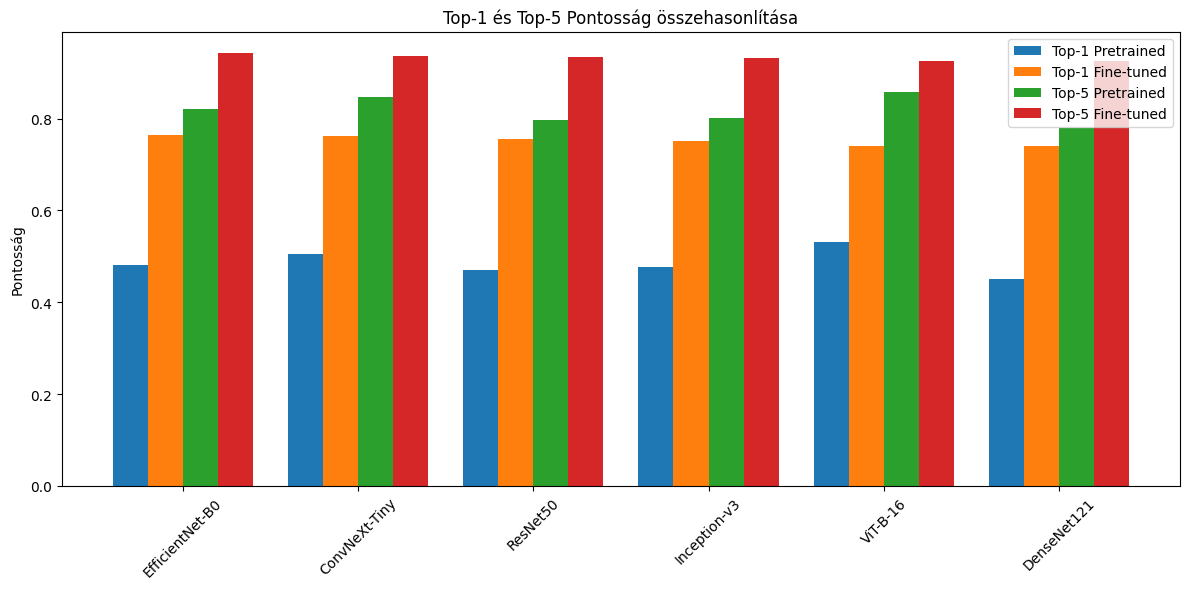
\includegraphics[width=1.0\textwidth]{images/phase02/phase02_summary_top1_vs_top5_pre_vs_fine.png}
        \caption{Top 1 és Top 5 pontosság összehasonlítása Pretrained és a Finetuned mérések között.}
        \label{fig:phase02_summary_top1_vs_top5_pre_vs_fine}
    \end{figure}

\subsection{Precision és Recall összehasonlítása Pretrained és a Finetuned mérések között.}
    \begin{figure}[H]
        \centering
        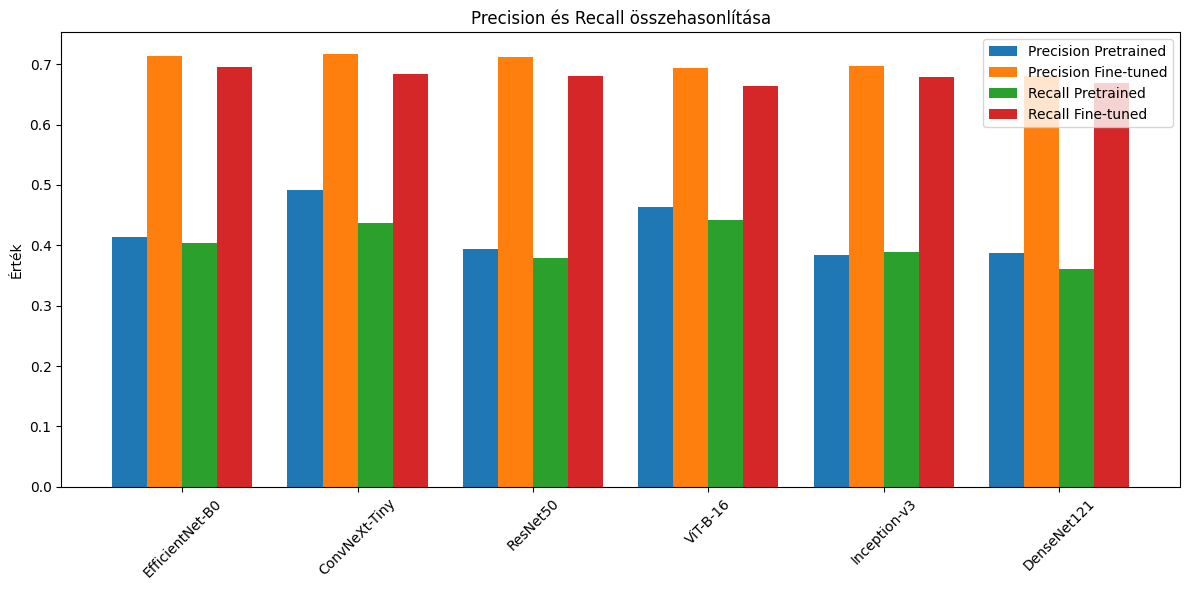
\includegraphics[width=1.0\textwidth]{images/phase02/phase02_summary_prec_vs_rec_pre_vs_fine.png}
        \caption{Precision és Recall összehasonlítása Pretrained és a Finetuned mérések között.}
        \label{fig:phase02_summary_prec_vs_rec_pre_vs_fine}
    \end{figure}

\subsection{F1 score összehasonlítása Pretrained és a Finetuned mérések között.}
    \begin{figure}[H]
        \centering
        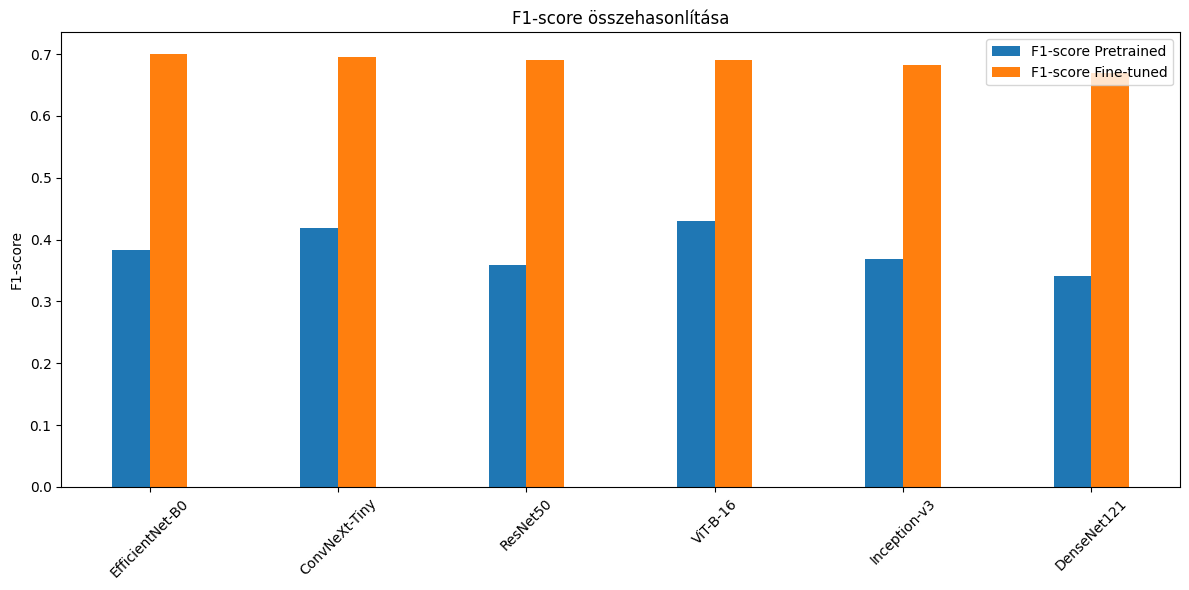
\includegraphics[width=1.0\textwidth]{images/phase02/phase02_summary_F1_pre_vs_fine.png}
        \caption{F1 score összehasonlítása Pretrained és a Finetuned mérések között.}
        \label{fig:phase02_summary_F1_pre_vs_fine}
    \end{figure}

\subsection{A Precision és a Fine-tuned modellek értékelése}
    A fenti eredmények alapján megállapítható, hogy a finomhangolt (fine-tuned) modellek jelentős teljesítményjavulást mutatnak a kiindulási, előképzett (pretrained) állapothoz képest. Különösen az EfficientNet-B0 és a ConvNeXt-Tiny modellek emelkednek ki, amelyek a legmagasabb Top-1 és Top-5 pontosságot érték el a finomhangolás után.

    A Precision, Recall és F1-score metrikák szintén javulást mutatnak minden modell esetében a finomhangolás hatására. Ez arra utal, hogy a modellek nemcsak pontosabbak lettek, hanem jobban képesek felismerni a releváns jellemzőket az adathalmazon.

    Az inference idő tekintetében a ViT-B-16 modell jelentősen hosszabb időt igényel

\subsection{Tanítási ciklusok elemzése}
Általános megfigyelések:
Tanítási pontosságban (Train Accuracy) ResNet50 (96.51\%) és ConvNeXt-Tiny (95.77\%) szerepeltek kiemelkedően.
Validációs pontosságban (Validation Accuracy) az EfficientNet-B0 (76.58\%) és NASNet (75.98\%) mutatták a legjobb eredményt.
A legtöbb modellnél overfitting (túlilleszkedés) jelentkezett: a Train Loss nagyon lecsökkent, miközben a Val Loss magas maradt (1 körül vagy felette).
NASNet csak 3 epoch alatt futott, mégis a legjobb vagy közel legjobb validációs eredményt érte el, ami hatékony tanulásra utal.
ViT-B/16 (Vision Transformer) és Inception-v3 bár jól tanultak (magas train acc), a validációs loss alapján nem tudtak igazán generalizálni.

Modellenként:
ResNet50: 
Nagyon erős tanítási eredmény, de látványos overfitting.
DenseNet121: 
Stabil fejlődés, viszont a validációs eredmény nem nőtt jelentősen a vége felé.
EfficientNet-B0: 
Legjobb tradeoff: relatíve jó tanulás + legjobb validáció.
ConvNeXt-Tiny: 
Nagyon jól tanult, de a validáció során hullámzó teljesítményt mutatott.
ViT-B/16: 
Transformer alapú architektúra itt nem volt erősebb, mint a CNN-ek.
Inception-v3: 
Stabil, de szintén overfitting jelei.
NASNet: 
Gyors, kevés epoch alatti hatékony tanulás. Figyelemre méltóan jó validációs pontosság.

\subsection{A Train és Validation loss alakulása modellenként.}
    \begin{figure}[H]
        \centering
        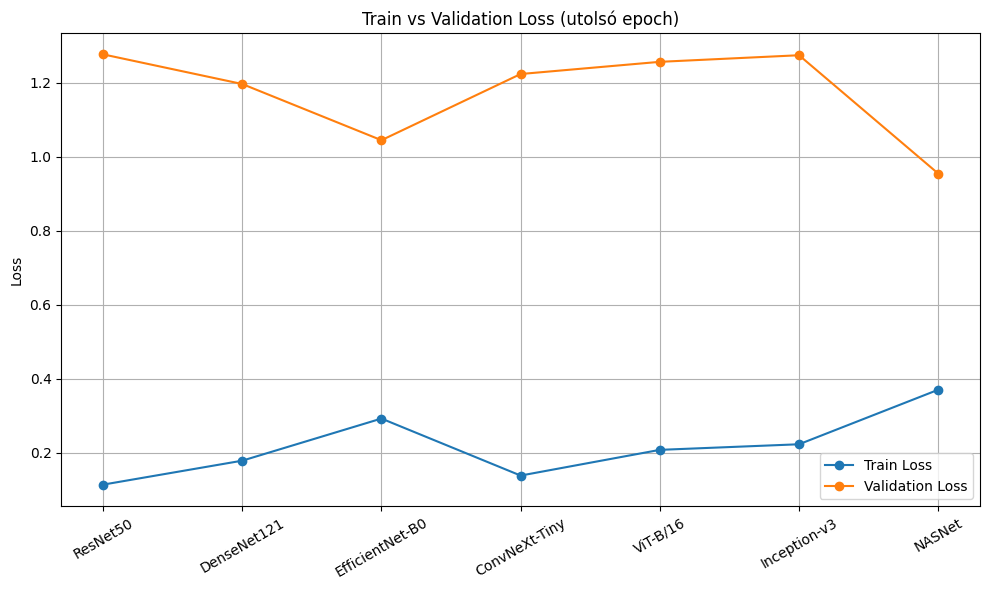
\includegraphics[width=1.0\textwidth]{images/phase02/phase2_summary_learning_stat_last_01.png}
        \caption{A Train és Validation loss alakulása modellenként.}
        \label{fig:phase2_summary_learning_stat_last_01.png}
    \end{figure}

\subsection{A Train és Validation accuracy alakulása modellenként.}
    \begin{figure}[H]
        \centering
        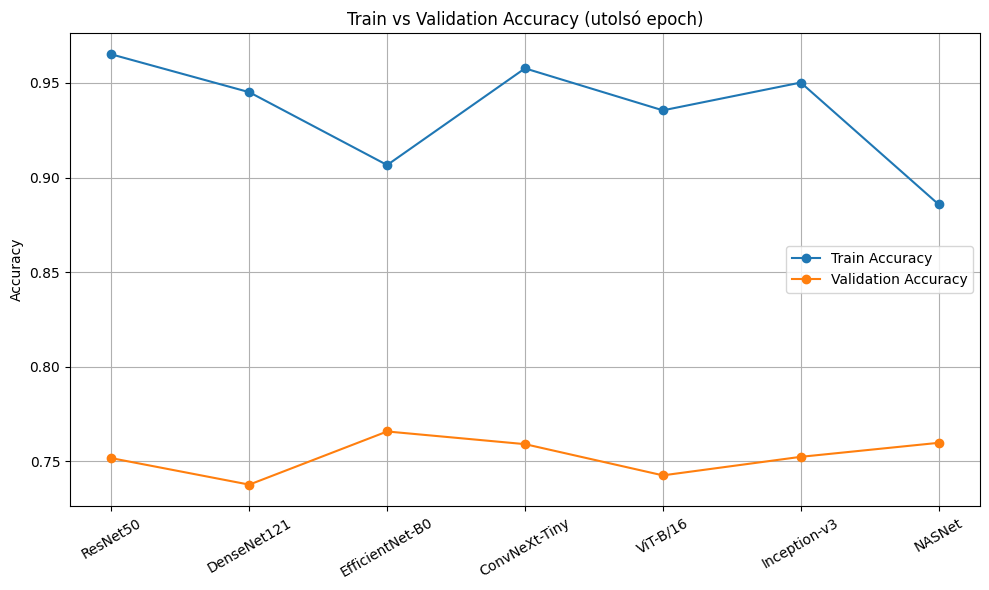
\includegraphics[width=1.0\textwidth]{images/phase02/phase2_summary_learning_stat_last_02.png}
        \caption{A Train és Validation accuracy alakulása modellenként.}
        \label{fig:phase2_summary_learning_stat_last_02.png}
    \end{figure}

\subsection{A Train és Validation loss alakulása modellenként epoch-ok szerint.}
    \begin{figure}[H]
        \centering
        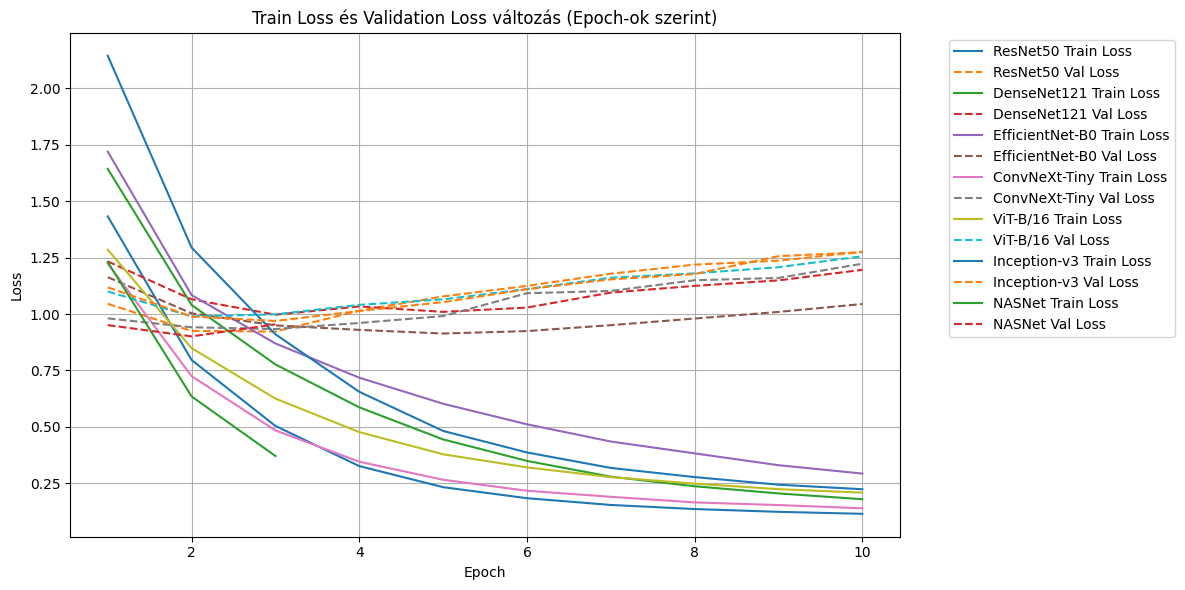
\includegraphics[width=1.0\textwidth]{images/phase02/phase2_summary_learning_stat_full_01.png}
        \caption{A Train és Validation loss alakulása modellenként epoch-ok szerint.}
        \label{fig:phase2_summary_learning_stat_last_01.png}
    \end{figure}

\subsection{A Train és Validation accuracy alakulása modellenként epoch-ok szerint.}
    \begin{figure}[H]
        \centering
        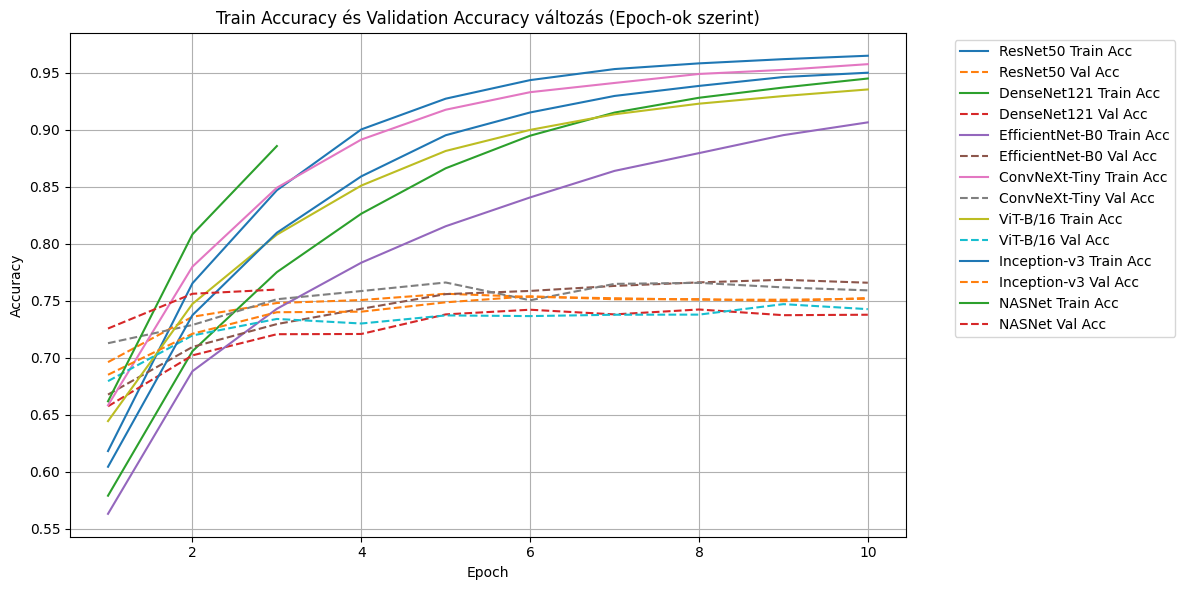
\includegraphics[width=1.0\textwidth]{images/phase02/phase2_summary_learning_stat_full_02.png}
        \caption{A Train és Validation accuracy alakulása modellenként epoch-ok szerint.}
        \label{fig:phase2_summary_learning_stat_last_02.png}
    \end{figure}

\subsection{A második fázis rövid szöveges értékelése}
    A második mérési fázis során a SBphotothemes180k [ImageNet114] adathalmazon végzett teljes tanítási folyamat után a különböző modellek teljesítményét értékeltük. Az alábbi megállapítások születtek:

    EfficientNet-B0 érte el a legmagasabb Top-1 pontosságot (76.49\%) és F1-score-t (70.01\%), miközben az inference ideje is versenyképes maradt. Ez alátámasztja az EfficientNet architektúra hatékonyságát és pontosságát, különösen a korlátozott erőforrásokkal rendelkező környezetekben.

    NASNet kiemelkedett a Top-5 pontosság terén (94.70\%) és a legmagasabb precizitást (71.80\%) érte el, ami a modell mély és összetett architektúrájának köszönhető. Azonban az inference ideje megegyezett más modellekével, ami azt jelzi, hogy a komplexitás nem feltétlenül jár együtt hosszabb feldolgozási idővel.

    ConvNeXt-Tiny és ResNet50 modellek kiegyensúlyozott teljesítményt mutattak, mind a pontosság, mind az inference idő tekintetében. Ez teszi őket megbízható választássá általános célú alkalmazásokhoz.

    ViT-B/16, bár transformer alapú modellként ígéretes, a jelenlegi adathalmazon nem tudta felülmúlni a CNN alapú modelleket. Az inference ideje is jelentősen hosszabb volt, ami korlátozhatja a valós idejű alkalmazásokban való használatát.

    Inception-v3 stabil teljesítményt nyújtott, különösen az F1-score (69.08\%) és az inference idő (25.11 sec) tekintetében, ami a modell érettségét és optimalizáltságát tükrözi.

    DenseNet121 hasonlóan jó eredményeket ért el, különösen a recall értékben (68.08\%), ami a modell hatékony információáramlását és mély kapcsolatokat kihasználó architektúráját mutatja.

    Összefoglalva, a teljes tanítási folyamat jelentős javulást eredményezett minden modell esetében a tanítás nélküli állapothoz képest. Az eredmények alapján az EfficientNet-B0 és a NASNet modellek kiemelkednek a pontosság és hatékonyság terén, míg a ConvNeXt-Tiny és a ResNet50 modellek megbízható és kiegyensúlyozott teljesítményt nyújtanak. A választás során figyelembe kell venni az alkalmazás specifikus igényeit, beleértve a pontosságot, a feldolgozási időt és az erőforrás-korlátokat.
